\documentclass{l4proj}

    
%==============================================================================

\usepackage{pdfpages} 
\begin{document}

%==============================================================================
%% METADATA
\title{Measuring QUIC performance: An analysis of Security and Connection Establishment in QUIC with comparison to TCP}
\author{Lara D'Agata}
\date{March 20, 2024}

\maketitle

%==============================================================================
%% ABSTRACT
\begin{abstract}

QUIC is a new transport layer protocol which has been in development since 2016, and has recently been deployed and finalised by the IETF in 2021 \citep{Iyen2021}. Consequently, there are not many studies available which analyse the performance of QUIC, and even less studies which take active measurements in a non-closed testing environment. Moreover, only a handful of papers explore the differences between QUIC and TCP, which is the most widespread transport protocol over the Internet currently. In order to bridge the gap between the deployment of QUIC and its related research, a measurement study has been performed by querying the top 1000 most popular URLs using both QUIC and TCP from multiple vantage points. The experiment conducted in this project is among the first to investigate the effects of the QUIC transport protocol on the establishment speed and security of connections, and compare QUIC to the more widely-used transport protocol, TCP. The results presented in this study show that QUIC generally performs better than TCP in most aspects of connection establishment. However, the difference between QUIC and TCP performance is not as large as QUIC promises, with TCP often performing better than QUIC in high latency networks.


\end{abstract}

%==============================================================================
%% ACKNOWLEDGEMENTS
\chapter*{Acknowledgements}

I would like to thank my supervisor Dr. Colin Perkins for taking on this project, and allowing me to conduct some interesting research. I would also like to express my thanks to PhD researchers Vivian Band, Elizabeth Boswell, and Mihail Yanev for supporting me throughout the year and for dedicating a lot of time and effort in responding to my questions.

%==============================================================================

% EDUCATION REUSE CONSENT FORM
\def\consentname {Lara D'Agata} 
\def\consentdate {March 20, 2024} 
\educationalconsent


%==============================================================================
\tableofcontents


%==================================================================================================================================
\chapter{Introduction}

\pagenumbering{arabic} 

\section{Motivation}

TCP has been the most widespread transport protocol across the Internet since its development forty years ago \citep{Postel1981}. However, with the recent development and deployment of QUIC, the ways in which we connect and transfer data over the Internet could see drastic changes in the near future. QUIC is a modern transport protocol developed by Google and finalised by the Internet Engineering Task Force (IETF) just a few years ago \citep{Iyen2021}. It represents a promising improvement to the currently available transport protocols, both in terms of speed and security of its connections. The creation of QUIC opens up the possibilities of development in the field of networking, laying the groundwork for the evolution of newer, more efficient transport protocols in the future. 

However, despite the encouraging prospect of faster, more secure connections over the Internet, QUIC does not yet benefit from the reliability and available documentation of older protocols like TCP. QUIC libraries and implementations are new and poorly documented, and support for bugs is limited. Moreover, the CPU usage in QUIC is very high compared to that of TCP, generating additional overhead in the network in which it operates \citep{Shreed2022}. It will take years before QUIC is as stable and performant as TLS over TCP: this project aims to measure the current state of QUIC's deployment and performance, in the hopes of encouraging its development.

\section{Research Aims}

The goal of this project is to understand how Internet transport protocols are changing, and to observe whether new protocols such as QUIC actually bring more benefits than costs to the changing Internet. In order to achieve this, an experiment was designed to observe the differences between QUIC and TCP operating over the Internet. The experiment collects data by taking active measurements of the top 1000 most popular URLs (as of January 2024) using both QUIC and TCP transport protocols from a specific testing environment, and analysing their performance, speed of connection establishment, and security parameters determined.

This measurement study aims to help the growth of available data regarding QUIC performance, in order to hopefully see a transition to QUIC as the new default transport protocol in the future. 

The main aim of this project is to investigate how TCP and QUIC correlate, and what effect they have on connection establishment and performance over the Internet. The following research questions will be addressed and discussed in this study.

\begin{itemize}
    \item {How is the security of a connection affected by the transport protocol used?}
    \item {How is the speed of connection establishment affected by the transport protocol used?}
    \item {How does the performance of a transport protocol vary depending on the location and configuration of the Client in a Client-Server connection?}
\end{itemize}


\section{Results Summary}

The results obtained from this project showed that QUIC does indeed show benefits to Internet connections, both in terms of speed and security. The vast majority of sites queried took less time to establish security parameters and reach the data transfer stage with QUIC compared to TCP. More QUIC connections were found to have established TLS ciphers than TCP connections, but QUIC connections also produced more TLS-related errors. Additionally, connections using QUIC were found to have a lower RTT, and faster duration for the connection establishment handshake.

Overall, the results obtained show that QUIC outperforms TCP in almost every aspect of connection establishment and security. Despite this, it was also found that for high-speed servers and networks with lower latency, TCP performs better than QUIC by a small margin.


\section{Dissertation Outline}

This dissertation is structured into six chapters: excluding the Introduction, they are structured as follows.

\subsubsection{Chapter 2: Background} This chapter will introduce the most significant notions relating to this project, such as providing an outline of the main features of both QUIC and TCP. Moreover, any existing research and related work in the field will be presented and discussed. 

\subsubsection{Chapter 3: Analysis \& Requirements} In this chapter, the gaps in existing research and related work will be addressed, which leads into the main aim of this project. The requirements for this project will be outlined in this chapter as well.

\subsubsection{Chapter 4: Experimental Design} Here, the details of the experiment will be explained and motivated. This chapter is divided into two main sections, relating to the data collection and data analysis stages of the experiment. Any design choices will be addressed, along with detailed explanations of the setup and implementation for the experiment.

\subsubsection{Chapter 5: Results} This chapter presents the results obtained and discusses their significance. Multiple visualisations are displayed to accompany the written discussion of the results. This chapter also contains a section evaluating the experiment, addressing its limitations and critiquing its validity.

\subsubsection{Chapter 6: Conclusion} In this chapter, the study concludes in a summary of the project and a reflection on the work done. Moreover, future work in this project's area will also be considered and discussed in this chapter.


%==================================================================================================================================
\chapter{Background}

This chapter will introduce and elaborate on previous work conducted in the area of this project. The different types of Internet Measurements that can be performed will be outlined, as well as those specifically relating to monitoring the activity of transport protocols. The Internet Protocol will be introduced along with a brief explanation of UDP. Additionally, the TCP and QUIC transport protocols as well as their relevant functionalities will be discussed, including Transport Layer Security and how it is relevant to this project. Moreover, the related work done in this area, along with any shortcomings, will be explored and discussed in this chapter.


\section{Internet Measurements}

Since its creation and consequent expansion across the world, the Internet has changed in numerous unpredictable ways which have altered the way we communicate and operate as a society. Everything about the Internet has undergone many changes over the years, such as the introduction of Network Address Translators (NATs) and firewalls, or the decline and eventual depletion of available IPv4 addresses which led to the introduction of IPv6. This dynamic and evolving nature of the Internet and its surrounding technologies inevitably leads to an ongoing increase in complexity of the network as a whole \citep{John2010}. The only realistic method for acquiring a better understanding of this Interconnected Network is to monitor its traffic: perhaps only in this way, by analysing the data obtained through measurements, will it be possible to find ways to improve the Internet. 

Internet traffic can be measured in various ways, each with different purposes and resulting outcomes. The different methods and best practices of Internet measurements are outlined in this section.

\subsubsection{Active vs Passive Measurements} This is the most common classification of Internet measurements. A passive measurement approach indicates the pure observation of existing Internet traffic, meaning that it is not intrusive and does not change existing traffic \citep{John2010}. On the other hand, active measurements involve the insertion of additional traffic into the current network in order to gain insight into certain network devices or properties. Active approaches may not be the best method to ascertain conclusions about Internet traffic, due to their intrusive nature which could disrupt the latency or congestion on the network. However, they are extremely useful in gaining insight about the workings of Internet communications, such as network latency to a particular destination, Internet routing paths, or link capacities and latencies along a particular Internet path \citep{William2001, Medi2005}.

\subsubsection{Online vs Offline Analysis} Network traffic can be analysed directly through the immediate processing of data: online analysis supports real-time data collection and analysis, which may contain visualisations of live traffic data. However, offline measurement approaches are intended only for real-time data collection and storage without the additional real-time analysis provided by online approaches. Once the traffic data is collected and stored using an offline measurement tool, it may be analysed: unlike online analysis, this method is not time-sensitive and provides the possibility of comparing network traffic collected at different times or locations. Moreover, once traffic data is collected and stored, it is possible to re-analyse it with different perspectives, and the collected dataset may be re-used for further analysis of Internet traffic \citep{John2010}.

\subsubsection{Packet-level Traces} Data regarding Internet traffic can be collected in various different ways. Network flows, for example, are used to observe condensed network information relevant to a specific network flow. These flows may be uni- or bidirectional, and represent a really good method for collecting summarised data regarding Internet traffic. On the other hand, packet-level traces represent a more in-depth view into the singular packets sent and received over a certain network: these may include any number of information from a single packet.

\subsection{The Internet Protocol (IP)}

In order to send data over the Internet, it is necessary to split that data into smaller pieces, or packets, so it can be manageable and easily transmissible. The Internet Protocol (IP) is a routing protocol for addressing data packets to send them to the correct destination over the Internet: each packet contains IP information which indicates where to send it. Data packets are processed differently depending on the transport protocol used in combination with IP: the most common transport protocols are the Transmission Control Protocol (TCP) and the User Datagram Protocol (UDP). 

\subsubsection{TCP/IP} TCP is a transport protocol which decides how data is sent and received over the Internet. Each packet that uses TCP in combination with IP is sent in order, and the recipient of the packets will acknowledge each packet which arrives to avoid missing packets in the process. TCP is reliable and will not send a packet unless the previous one has been received and acknowledged, meaning that the transmission of data via TCP/IP can take a long time if there are missing packets \citep{Postel1981}.

\subsubsection{UDP/IP} UDP is a widely used transport protocol, it is faster than TCP but less reliable. UDP does not acknowledge each packet at the recipient, meaning that not all packets are sure to be delivered correctly. Moreover, not all packets are necessarily delivered in order. UDP also does not establish a connection between sender and recipient before initiating data transmission \citep{Postel1980}.

\subsection{Measuring Transport Protocols}

Transport protocols are very restricted in how they are permitted to operate in today's Internet. Among other Internet limitations, the introduction of middleboxes such as firewalls and NATs poses a definite challenge in the development and deployment of better transport protocols, as the security and functionality of the Internet could be at risk. New transport protocols have to consider the environments in which they could be used, as well as the scale of their deployment: they need to update and evolve as the Internet itself changes. This poses a considerable challenge in the design and implementation of any new transport protocols, the analysis of which is exceptionally valuable when observing behaviour across different environments and Internet topologies \citep{Fair2021}.

\subsubsection{Middlebox Interactions} Middleboxes are smart network entities such as firewalls, address translators, and proxies, which are integral in today's Internet architecture. Middleboxes are used for various purposes, such as maintaining security over the Internet, increasing performance of transport protocols, or address translation. Despite the fundamental role played by middleboxes across the Internet, these entities are not easily updated, which makes it very difficult to keep up with new technologies, including new transport protocols \citep{Allman2003}.
The performance of transport protocols over the Internet can be greatly affected by middleboxes, which can represent hidden points of failure in the network. Some middleboxes are able to modify the contents of an IP packet, as well as diverting a packet from its original destination: these instances of tampering with IP packets indicate an infringement of the uninterrupted transfer of packets across the destination \citep{Medi2005}. These changes may have an unpredictable effect on the functionality, performance, and reliability, of transport protocols.

\subsubsection{Round Trip Time} Another important property to measure regarding Internet transport protocols in the Round Trip Time (RTT) of the connections they establish. The RTT is defined as a "measure of the elapsed time between sending a data octet with a particular sequence number and receiving an acknowledgment that covers that sequence number [...]" \citep{Postel1981}. The RTT of a particular connection represents the time taken by a transport protocol to send and receive a packet: this is incredibly important to analyse, because this information can indicate many things about both endpoints in a connection. For example, a longer RTT may indicate that the Client and Server are in distant physical locations, or high traffic across a particular network path. Additionally, RTT can give an insight into how quickly a transport protocol is able to transfer packets between endpoints, thus providing insight into the performance and efficiency of transport protocols.


\section{TLS (Transport Layer Security)}

Transport Layer Security (TLS) allows connections established over the Internet to communicate while preventing security vulnerabilities such as eavesdropping, tampering, and message forgery \citep{Resc2018}. TLS supports a handshake protocol which allows endpoints to negotiate security parameters, including protocol version and cryptographic algorithms.

\subsubsection{Handshake Protocol} A TLS handshake involves a hybrid approach of public-key and symmetric encryption mechanisms to exchange keys for encrypting messages with. Additionally, the key exchange step is necessary to determine the security capabilities of the two endpoints. Then, the TLS handshake involves a negotiation of certain cryptographic parameters, such as cipher suites, signature algorithms, and a pre-shared key extension \citep{Resc2018}. 

\subsection{TLS Cipher Suites}

Cipher Suites are a set of instructions that enable a secure network connection through TLS. The cipher suite specified during a connection provides a set of algorithms and protocols necessary to secure communication between the client and server \citep{Siman2023}. More specifically, the TLS cipher suite specifies firstly the key exchange algorithm, which can be ECDHE or CHACHA20, then the authentication algorithm, which can be RSA or ECDSA. After the "WITH" keyword, the cipher specifies  its algorithm, strength, and mode: for example, AES\_128\_GCM would indicate the use of an AES algorithm with key size 128-bit, using Galois/Counter mode. This is followed by a Pseudo-random function or message authentication code, such as a version of SHA (Secure Hash Algorithm).

This section will elaborate on some common key exchange and authentication algorithms, as well as outlining common modes and encryption algorithms that are relevant in the context of this experiment. 

\subsubsection{Advanced Encryption Standard (AES)}

AES is a symmetric encryption algorithm selected by the National Institute of Standards and Technology (NIST) to replace the older DES (Data Encryption Standard). AES operates on fixed-size blocks of data (128 bits), and it supports key sizes of 128, 192, or 256 bits. For example, in AES256, the algorithm uses a 256-bit key for encryption and decryption.

\subsubsection{Galois/Counter Mode (GCM)}

GCM is a mode of operation for block ciphers (like AES) that provides both encryption and message authentication. GCM combines the counter mode of encryption with the Galois/Counter Mode (GCM) authentication algorithm. It offers high performance, parallelism, and strong security \citep{McGrew2005}.

\subsubsection{Ephemeral Elliptic Curve Diffie-Hellman (ECDHE)}

 Ephemeral Diffie-Hellman key exchange ensures that the session keys are ephemeral and are not derived from long-term keys, providing forward secrecy \citep{Siman2023}. It is a widely adopted choice for securing communications in modern cryptographic protocols like TLS.

 \subsubsection{Rivest-Shamir-Adleman (RSA)}

 RSA is one of the earliest and most widely used public-key cryptographic algorithms. It uses asymmetric encryption, and is commonly employed for secure data transmission, digital signatures, and key exchange in various cryptographic protocols \citep{Zhou2011}.

 \subsubsection{Elliptic Curve Digital Signature Algorithm (ECDSA)}
 
 ECDSA is a cryptographic algorithm used for generating digital signatures based on elliptic curve cryptography \citep{John2001}. ECDSA is widely used in various cryptographic applications, including digital signatures for authentication and integrity verification.

\subsubsection{ChaCha20 and Poly1305}

ChaCha20 is a stream cipher which uses a 256-bit key. Poly1305 is a one-time authenticator which takes a 32-byte one-time key and a message and produces a 16-byte tag which is used to authenticate the message \citep{Nir2018}.

\subsection{TLS Alerts}

The TLS record layer supports various content types, including alert messages. These messages are called TLS Alerts and indicate the severity of an issue, whether it's a warning or fatal, and provide a brief description of the type of alert. If a TLS Alert message is marked as fatal, it leads to the abrupt termination of the connection \citep{Resc2018}. 


\section{UDP}

The User Datagram Protocol (UDP) is a connectionless, unreliable, best-effort service for packet delivery over the Internet. UDP is the simplest of the available transport protocols, as it has no mechanism for congestion control and does not send packets in order \citep{Postel1980}. Moreover, UDP does not need to establish a connection before initiating data transfer, so there is no added latency for connection establishment.

Applications which use UDP as a transport protocol have no end-to-end integrity, flow control, or congestion control. However, UDP is faster than TCP and usually is able tolerate the loss of some data \citep{Rahoum2020}. 


\section{TCP}

The most commonly used transport layer protocol today (2024) is the Transmission Control Protocol (TCP). TCP is a connection-oriented protocol which is based on positive acknowledgements: when a packet is sent over a TCP connection, it requires some form of acknowledgement from the other endpoint in the connection. Moreover, TCP offers a congestion avoidance mechanism to reduce the transmission rate when the network becomes overloaded \citep{Rahoum2020}. It is the first transport protocol to have introduced some form of congestion control over the network, allowing the Internet to become what it is today. TCP has been operational for around forty years, and has been proven to be an extremely reliable transport protocol. According to its original specification, TCP is a "connection-oriented, end-to-end reliable protocol designed to fit into a layered hierarchy of protocols which support multi-network applications." \citep{Postel1981}, meaning that it was designed to be adaptable to different network conditions and failures \citep{Rahoum2020}. 

\subsubsection{TCP/TLS} Before a Client and Server can transfer data among themselves through a dedicated TCP connection, they must first establish a connection through connection establishment and security handshakes. The connection establishment or transport handshake in TCP is more commonly referred to as the "three-way handshake", and it involves sending three packets between the Client and Server to establish the parameters for the connection \citep{Rahoum2020}. Immediately after the three-way handshake, the TLS handshake needs to occur in order to establish security parameters over the connection that has just been established. After the completion of both handshakes, the Client and Server can transfer data safely over the TCP connection. Figure ~\ref{fig:TCPTLSvsQUIC_handshakes} shows a generalised outline of the number of packets which need to be sent in order to establish a secure connection with TCP and TLS.


\section{QUIC}

QUIC is a brand new transport layer protocol which has been recently deployed and can now be used by applications to transmit data over the Internet. QUIC is an encrypted, multiplexed, and low-latency transport protocol, especially designed improve transport performance for HTTPS traffic and facilitate its own deployment. The creation of QUIC promotes the continued evolution of transport mechanisms, while introducing some groundbreaking changes to the ways in which transport protocols can operate over the Internet. QUIC aims to effectively replace TCP as the new default for establishing connections and transferring data over the Internet.

In this section, the most significant properties and features of QUIC are briefly outlined and explained.

\subsubsection{Running Over UDP} QUIC was built over UDP in order to ease end-system deployment in user-space applications and expedite its deployment. This signifies that QUIC can operate at higher speeds than TCP. Building over UDP has the additional benefit of allowing QUIC packets to securely traverse middleboxes without being blocked by firewalls. 

\subsubsection{Combined Handshake} QUIC connections reduce latency by overlapping the transport and TLS security handshakes into a single handshake which establishes a secure connection in only one round trip. This is extremely useful in reducing the time taken before data can be transferred across a connection, and limits the round trips necessary in order to establish a cryptographically secure transport connection \citep{Lang2017}. Figure ~\ref{fig:TCPTLSvsQUIC_handshakes} shows how QUIC's combined transport and security handshake reduces the number of round trips between Client and Server compares to TCP/TLS.

\subsubsection{Dedicated Streams} A QUIC connection comprises of QUIC packets sent within UDP datagrams, where each QUIC packet starts with a header and contains one or more frames. QUIC provides a dedicated reliable stream to allow faster connection establishment. QUIC streams provide a reliable and bidirectional connection stream which may be used to frame an encrypted payload of any size \citep{Iyen2021}. Streams in QUIC are extremely lightweight, meaning that it is possible to initialise a new stream for each message, no matter how small. Moreover, these streams can be cancelled at any point without breaking the connection, but QUIC does not re-transmit data from such streams \citep{Lang2017}. 

\subsubsection{Head-of-Line Blocking} TCP always delivers data to the application in a continuous ordered sequence, and when a packet is lost during a connection, the TCP receiver will wait for the missing data to be re-transmitted. This phenomenon is referred to as Head-of-Line (HoL) blocking, and can cause a significant increase in latency over the connection: the dedicated streams provided in QUIC connections aim to completely avoid this problem. Order is not preserved between streams in a QUIC connection: one stream might be blocked waiting for a re-transmission, while other streams continue to deliver data without loss. Data from different streams is sent and received independently, and is delivered reliably and in-order: whether packet loss affects one or more streams depends on how the sender chooses to distribute the stream data between packets. Through a careful use of streams in a QUIC connection, is it possible to greatly reduce the duration of HoL blocking \citep{Lang2017}.


\begin{figure}
    \centering
    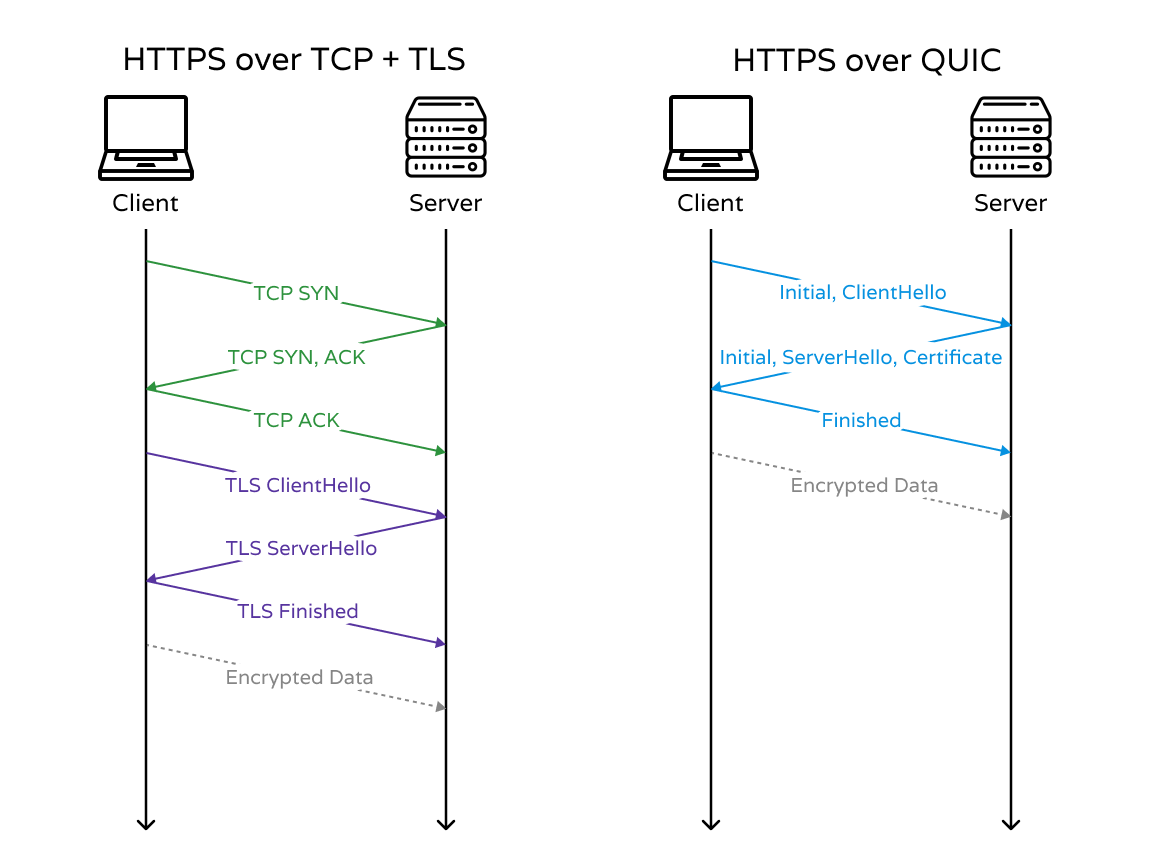
\includegraphics[width=0.75\linewidth]{images/connectionEstablishmentHandshakes.png}
    \caption{Visualisation of the different transport and security handshakes in a TCP/TLS connection compared to a QUIC connection. TCP transport handshake is depicted in green, TLS handshake in purple, and QUIC combined handshake in blue.}
    \label{fig:TCPTLSvsQUIC_handshakes}
\end{figure}


\subsubsection{Connection Errors} Endpoints in a QUIC connection report any errors to each other. \citet{Iyen2021} describes two different types of error handling in QUIC: connection and stream errors. Stream errors occur on the application-level and only affect a single stream without tampering with the integrity of the connection as a whole. Connection errors often cause the connection to be unusable: this could happen after a violation of protocol semantics, or a corruption of state which affects the connection \citep{Iyen2021}. These errors could be related to the security of connections, and therefore it is important to analyse and understand why they occur.

\subsubsection{Encryption and Forward Secrecy} QUIC provides encryption by default through the use of TLS to establish security parameters, allowing all messages exchanges by the Client and Server across a connection to remain encrypted. QUIC security is based on the Diffie-Hellman key exchange to generate ephemeral public and private keys: this also allows forward secrecy in connections by establishing new encryption keys for each data exchange, protecting all past activity. This encryption mechanism also provides effective protection from eavesdropping and tampering by third parties. Additionally, by reducing the amount of unencrypted data in its packet headers, QUIC connections present a challenge for any adversary who wishes to monitor users \citep{Liu2023}. 

\subsubsection{QUIC Implementations} Although QUIC was recently finalised, some design choices were not defined by the IETF and can be specified in different ways. Features such as congestion control, multiple streams, and packet size are left open to the developer and can be changed depending on the required parameters of connections at specific endpoints. Therefore, different implementations of QUIC have been developed in order to specify the parameters of these features, allowing QUIC to operate in multiple ways. \citet{Hertel2022} explores the different QUIC implementations that have been written by developers since the finalisation of QUIC in 2021, and have found that there is a large diversity in the technologies used and features implemented.

\section{Measuring QUIC Behaviour}

In this section, multiple studies analysing QUIC performance and security will be presented and discussed. Given that QUIC is a newly developed transport protocol, not many such studies exist. However, the papers introduced below represent the most significant studies conducted so far relating to analysing QUIC's performance.

\subsection{QUIC performance}

\cite{Ruth2018}  presented the first broad assessment of QUIC by probing the entire IPv4 address space, and found that many domains were capable of supporting QUIC. However, its infrastructure size does not reflect the share of Internet traffic: despite operating a similar number of QUIC-supporting IP addresses, Google accounts almost entirely for QUIC's traffic share compared to Akamai \citep{Ruth2018} . This tells us that, despite there being many IPs that are able to support QUIC connections, most of them are hosted by one singular entity (Google) which may hold a monopoly over these connections if QUIC were to be deployed. 

On the other hand, some studies have tried to break QUIC and find its weaknesses. These studies are just as important if not more so than those supporting QUIC: given that the transport protocol is still under development, it is essential to expand its documentation by finding bugs or other inconsistencies in its performance. One such study by \cite{Yu2021}  found that QUIC’s removal of head-of-line blocking has little impact on web-page performance in practice. They showed that, despite inherent advantages over TCP in terms of latency, versatility, and application-layer simplicity, QUIC suffers the cost of high implementation overhead which leads to performance inconsistencies across its different implementations. This is important because it shows that the worldwide deployment of QUIC may not necessarily lead to improvements in overall network or application performance in practice. 

\subsection{Security in QUIC Connections}

\citet{Fisch2014} conducted an analysis of the QUIC transport protocol by using a security model. They found that QUIC can be considered an adequately secure multi-stage key exchange protocol, showing strong security properties despite its low complexity. Although QUIC does meet the suggested standards for security of transport protocols, \citet{Fisch2014} suggest that a few changes would be beneficial to implement in QUIC in order to improve its security.

Moreover, a study by \citet{Lychev2015} found that the key exchange in QUIC connections cannot be built upon. Therefore, QUIC’s security implementation is not independent from the key exchange phases and, because of this, treating multiple stages of key exchange is not possible in QUIC. This is just one of the few potential security risks with the QUIC transport protocol that may be encountered in the future.

\citet{Soni2021} recently conducted a significant study regarding the security of QUIC connections. Multiple security concerns were discovered, including forward secrecy, as well as replay and denial-of-service (DoS) attacks. It was found that QUIC does not provide forward secrecy at all, and that QUIC's multiple attack-prevention mechanisms are still under analysis and therefore do not yet achieve their required goal.

\subsection{Comparing QUIC to TCP}

A recent study by \citet{Wang2018} investigated the performance of QUIC from within a Linux kernel, and compared it to TCP's performance. In order to compare the two transport protocols fairly, they created a closed testing environment between two virtual machines (acting as Client and Server) and operated the connections on a custom-built WiFi testbed. This study clearly showed that QUIC outperforms TCP in almost every case, especially in networks with low latency and high packet loss rate. This paper provides a compelling insight into the difference between QUIC and TCP, showing that QUIC does propose a major improvement in terms of speed and latency. 

Another study looking at general performance by \citep{Kakh2017} found that QUIC performance tends to be at least as good as TCP performance. Although generally QUIC outperforms TCP, various issues were identified relating window sizes, packet re-ordering, and multiplexing a large number of streams for small objects. Moreover, QUIC's performance largely diminishes when observed over cellular networks compared to TCP.

\citet{Grat2016} performed an important study in comparing QUIC and TCP. It was found that, although Google claimed that "QUIC performs significantly better for slow connections with high latency and performs as good as TCP for fast connections with a low latency" \citep{Iyen2015}. However, the measurements taken by \citet{Grat2016} show that QUIC only performs better than TCP in networks with high latency and low bandwidth. However, TCP was found to perform better than QUIC where the network had high bandwidth and low latency. The only real advantage of QUIC found in this study was the 0-RTT handshake for repeated connections, and the stream multiplexing mechanism which is not present in TCP.

\citet{Nepomu2018} conducted a very prominent study to compare the speed and overall performance of QUIC and TCP. The web page load times were measured using both protocols, and then compared to analyse the difference in speed. It was found that, for connections in which the cache was disabled, TCP actually performed better in most cases. Considering all experiments, it was shown that QUIC only provided a better page load time for less than 40\% of the web pages queried. It was supposed that this effect could be due to the low support for QUIC over the Internet, but this is unsure. Moreover, enabling cache produced a much higher improvement in speed for TCP that it did in QUIC, indicating that TCP could still have better performance in terms of speed compared to QUIC.

\section{Summary}

In this chapter, the Internet standards and technologies used in this project have been introduced. 

Being the most widely-used transport protocol, TCP is reliable and connection-oriented. In a TCP connection, data is transferred in order on a single byte stream, whereas QUIC provides a secure, multiplexed connection which operates on multiple concurrent byte streams. TCP requires a TLS handshake in addition to its own transport handshake in order to establish a secure connection, meaning that the duration of connection establishment is equivalent to two RTTs. However, QUIC uses a combined transport and security handshake to establish all parameters necessary for a connection in a single round trip, making it much faster than TCP. 

According to the existing research which has been conducted in the field, it is unknown yet whether QUIC actually establishes secure parameters correctly. Moreover, although researchers have found QUIC to be generally faster than TCP, not enough studies have been conducted yet in order to come to a definitive conclusion regarding the actual performance of QUIC.


%==================================================================================================================================
\chapter{Analysis \& Requirements}

This chapter introduces the problems which this project aims to solve, referencing any gaps in the related research. Afterwards, the main aims of this project will be presented, followed by an explanation of the prerequisites and initial requirements for the project. 

\section{Problems with Existing Research}

\subsubsection{Lack of Research} Given that QUIC was first proposed in 2016 by Google \citep{Lang2017} and formally adopted as a standard by the IETF only in 2021 \citep{Iyen2021}, the number of studies measuring QUIC performance are extremely limited. Recently, Internet traffic has been rapidly moving towards QUIC, and there is great demand for the rest of the Internet to do the same. However, the research community is struggling to catch up with the increasing deployment and distribution of QUIC: not enough papers have been investigating QUIC's behaviour, or the effects that QUIC will have on the current Internet. Moreover, studies such as the one by \citet{Soni2021} show that there are still many security vulnerabilities to be considered with the use of QUIC. This indicates that the research surrounding QUIC performance and security has not yet been fully explored. It has therefore become increasingly important to perform as much research in this area as possible in order to accelerate this process, and possibly deploy QUIC on a global scale. For the moment, it is difficult to say whether QUIC will actually have a positive impact on latency and performance of connections across the Internet once fully deployed.

\subsubsection{Lack of Investigation in Real-World Environment} Studies such as the one performed by \citet{Wang2018} provide compelling insight into the difference between QUIC and TCP. However, having performed the experiment in a closed testing environment, this study does not observe QUIC operating over the Internet in a real-life scenario: if QUIC behaved a certain way in a closed environment, it does not follow directly that its behaviour on the Internet will be the same. Other studies such as the one by \citet{Nepomu2018} provide significant insight into QUIC's performance in the real-world. Despite measurements over the Internet being the most accurate method of identifying the practical shortcomings of a transport protocol, there are almost no studies today which investigate QUIC in a non-closed environment. Although there are many reasons for this, such as the extremely recent release of QUIC as a usable transport protocol on the Internet, it is crucial to analyse the performance of QUIC outside of a closed testing environment.

\subsubsection{Lack of Comparison Studies} Most studies observing QUIC's performance tend to focus on how QUIC operates individually, measuring its functionality as a standalone transport protocol. However, in order to fairly assess its actual performance, it is necessary to compare QUIC with the current standard. Being the most commonly used transport protocol in today's Internet, TCP makes for a perfect baseline for comparing QUIC to. It is extremely important to compare QUIC to an efficient, fast, and reliable transport protocol in order to test it properly and make sure whether it really achieves everything that it promises. It is equally important to compare QUIC to a transport protocol which is widely used: if QUIC is to replace TCP in the near future as the main transport protocol for all sites, the switch should represent an improvement on the current Internet, and not a setback. Therefore, comparing QUIC with TCP can allow us to gain insight into whether a possible switch to QUIC as a new standard transport protocol would actually be beneficial.

\section{Aim of this Project}

This project aims to address the gaps in existing research by conducting an experiment which measures the actual performance of QUIC operating in today's Internet, as well as recording any security vulnerabilities encountered. Furthermore, the experiment conducted in this study will collect data for both QUIC and TCP in order to fairly assess QUIC's performance and security. 


\section{Project Requirements}

The goal of this project is to compare QUIC performance and security to that of TCP. In order to achieve this, an experiment was conducted to query the most popular URLs over the Internet using both QUIC and TCP, and obtaining all metadata relating to those connections. 

It was essential for this project to conduct measurements from more than one location in order to investigate the effect of different Internet paths on the performance of QUIC, and the effect of different router bandwidth on the speed of QUIC connections. Moreover, the investigation of QUIC in a real-world environment is a very important aspect of this project, therefore the measurements were conducted actively from each location. Security parameters were also analysed in order to investigate the security configurations of QUIC connections, given than multiple studies have uncovered various possible security vulnerabilities in QUIC, such as the study by \citet{Soni2021}. It was essential to record TLS ciphers for comparing the security configurations of both QUIC and TCP, given the lack of existing studies which compare the two. Additionally, since there is a shortage of comparison studies regarding QUIC performance as well, it was necessary for this experiment to record the time taken to establish each connection and test the speed and overall performance of QUIC, and compare it to the performance of TCP. 

Some additional features which were collected and analysed in addition to the above are: a comparison of average RTTs, connection errors, TLS alerts, and the difference in transport and security handshakes for both QUIC and TCP. 

To summarise, the essential must-have aspects of this project are:

\begin{itemize}
    \item {Writing a bash script to gather data for both QUIC and TCP connections.}
    \item {Using the bash script: querying an updated list of most popular 1000 URLs using both QUIC and TCP.}
    \item {Gathering data from more than one location, possibly with variying specifications.}
    \item {Analyse the collected data to show TLS versions and ciphers to observe \textbf{security}.}
    \item {Analyse the collected data to show connection establishment times to observe \textbf{speed and performance}.}
\end{itemize}

The non-essential aspects of this project are:
\begin{itemize}
    \item {Obtaining a comparison of Round Trip Times between QUIC and TCP connections.}
    \item {A discussion regarding connection errors and TLS alerts found.}
    \item {An analysis of the difference between transport and security handshakes in QUIC compared to TCP.}
    \item {Using a cloud platform, such as RipeAtlas or DigitalOcean, to run the bash script from many vantage points in different regions for a more in-depth analysis of how location affects performance.}
\end{itemize}

\section{Summary}

In this section, the various problems with existing research have been explored: these include the overall shortage of research in this field, as well as the lack of testing QUIC in a non-closed environment, and many studies avoiding comparisons between QUIC and TCP. Moreover, the aims for this project have been clearly defined as adding to the pool of existing research studies by conducting accurate and fair measurements on the performance of QUIC. The requirements for this project have been introduced, and will be addressed in the implementation of the experiment.

%==================================================================================================================================
\chapter{Experimental Design}

In this chapter, the details of the experiment and its design will be outlined in detail in order to ensure the reproducibility of this experiment. The code for this project is stored in a GitHub repository \footnote{https://github.com/laradagata/l4project} and is publicly accessible. 


\section{Data Collection}

In this section, the details of the data collection stage of the experiment will be outlined. The technologies used, the setup of the testing environment, the installation of the necessary dependencies, and the details of the packet capture script will be introduced and discussed below.

\subsection{Overview} 

The data collection for this experiment was conducted on an Ubuntu virtual machine (VM) on the Oracle Virtualbox platform: this was done to allow very precise control of the allocated memory space and resources. Additionally, conducting the measurements and data gathering on a Linux VM allowed the use of \emph{tcpdump} as a data collection tool, which was extremely useful in generating accurate data from the measured connections. The metadata for each connection was collected by running a script which establishes the connection and queries the site using both QUIC and TCP transport protocols, where each site is taken from a list of current most popular URLs. The packets exchanged during each connection were recorded individually and stored in separate files for the subsequent data analysis. Querying each site using \emph{curl}\footnote{https://github.com/curl/curl} was sufficient to gather enough information for the TCP connections. However, since the packets captured in QUIC connections mostly have encrypted packet headers, it was necessary to utilise a QUIC implementation to query the sites using QUIC instead of \emph{curl}. The data was collected from two distinct locations, one of which was representative of a home router, and the other a high-speed server: a Linux VM was used at both locations to query the sites.

\subsubsection{Cloudflare \emph{quiche} Implementation} The Cloudflare implementation of \emph{quiche} is written in Rust and hosted on GitHib in a public repository\footnote{https://github.com/cloudflare/quiche}. This implementation of QUIC was developed by Cloudflare to enable HTTP/3 support on their servers. The extensive documentation available for \emph{quiche} is what makes it an attractive implementation to use, as its repository provides a comprehensive guide on how to build and configure the QUIC implementation to send/receive packets. The wiki of its GitHub repository also includes a vast archive of information relating to the structures and functions used in this implementation, along with detailed descriptions of each technology. One of the main congestion control algorithms supported by Cloudflare's implementation of \emph{quiche} is CUBIC, which is one of the most popular congestion control algorithms used in production \citep{Hertel2022}. Being one of the most widely-used and well-documented implementations of QUIC, Cloudflare's \emph{quiche} was chosen for this project, in order to obtain the most accurate data possible and to generate the biggest possible dataset.

\subsubsection{Majestic Million Top URLs} In order to accurately obtain a list of the top 1000 URLs to query during the experiment, the Majestic Million\footnote{https://majestic.com/reports/majestic-million} list of top URLs was utilised. This software is free to use and generates an updated list of the most popular URLs. The list was downloaded less than a week before conducting the experiment, ensuring the most accurate list possible during the packet capture.

\subsubsection{Packet Sniffing with \emph{tcpdump}} To capture data regarding the packets exchanged in each connection, it was necessary to use a packet sniffing tool. For this experiment, \emph{tcpdump} was chosen for the packet capture as it is "one of the finest and lightest network traffic capturing tools [which is] freely available" \citep{Goyal2017}. Aside from being compatible with the Linux OS and can be easily used in the virtual machine created, \emph{tcpdump} also provides several different options for viewing and storing the packets captured.

\subsubsection{Logging QUIC metadata using \emph{qlog}} As outlined by \citet{Marx2024qlog}, \emph{qlog} is an extensible high-level schema for a standardised logging format, which benefits from common analysis methods and tooling. \emph{qlog} is independent from the QUIC implementation used, and is used to provide amenities and default characteristics used by each logging file for improved readability and easy analysis \citep{Marx2024qlog}. In this experiment, \emph{qlog} files are obtained through querying sites with \emph{quiche-client}, and are used as a logging file format in which to store all data relating to QUIC connections.

\subsection{Testbed Setup}

The setup for the testbed is based on that of other similar studies, such as the experiments performed by \citet{Wang2018} in comparing QUIC and TCP performance. A Linux virtual machine was created using the Oracle virtualbox platform, which was used to represent the Client-side of the connections, querying each of the 1000 top URLs and gathering their related information.

The virtual machine created for this experiment used the following emulated configuration:
\begin{itemize}
    \item {10 core processor units (CPUs) capped at 100\% host machine core use.}
    \item {10000 MB of RAM.}
    \item {Intel PRO/1000 MT Desktop NAT adapter.}
\end{itemize}
This virtual machine ran on a host computer with an 12th Gen Intel(R) Core(TM) i7-1260P with 24 cores running at 2.10 GHz and 16GB of RAM. The implementation of the VM is based on the Linux 6.5.0 kernel of Ubuntu 22.04. This configuration ensures that the comparison of connections created by both QUIC and TCP takes place in a fair and isolated environment.

\subsection{Locations}

The data collection process was conducted on two different machines in order to investigate the effect of distance and differing Internet paths on the performance of QUIC and TCP. For the scope of this project, it was only possible to run the experiment from two locations. However, despite the limited number of different vantage points used, the two locations in which the packet capture script was run have very different specifications and can be representative of two types of connection.

\subsubsection{Location 1} This location represents a home router. The measurements taken at this location represent connections established through a residential WiFi network and passing through a router with an estimated download speed between 64.00 Mbps and 73.60 Mbps, with a minimum guaranteed download speed of 57.18 Mbps and upload speed of 14.00 Mbps.

\subsubsection{Location 2} This location represents a high-speed server located in the Department of Computing Science at the University of Glasgow. This server was accessed through the virtual machine at Location 1 by ssh'ing into the server at Location 2: this was made possible by granting SSH access to the virtual machine at Location 1.

\subsection{Installing Dependencies}

The necessary dependencies were installed onto the virtual machine using a Bash script \footnote{This script can be found in the GitHub repository for this project in \emph{/src/main/setup/} and is named \emph{setup.sh}}. The most important dependency used for this experiment was the QUIC implementation \emph{quiche}, the repository of which had to be cloned and built. Additionally, a rust compiler had to be installed in order to use \emph{quiche} to extract \emph{qlog} files for analysing the QUIC connections. 

\subsection{Packet Capture Script}

The data collection script is written in Bash \footnote{This script can be found in the GitHub repository for this project in \emph{/src/main/} and is named \emph{packetCapture.sh}} to be compatible with the Linux OS of the virtual machine. Listing ~\ref{lst:quicdata} is a code fragment from the packet capture script, detailing how the URLs were queried using QUIC and the data relating to each connection was stored in separate files.

\subsubsection{Preventing Data Overlap} Given that the packet capture script is querying 1000 URLs within the same loop, it is important to distinguish between the different connections, otherwise there will be no guarantee that the data generated and stored for a certain URL will contain data strictly pertaining to the connection to that specific URL. In order to mitigate this issue, a \emph{port\_num} variable was initiated in the script and incremented at every iteration of the for loop: this can be seen in line 29 of Listing ~\ref{lst:quicdata}. In this way, the source port used to query the website will be different for each URL, and when opening \emph{tcpdump} it is possible to specify the port to observe. This allows any data generated for a specific site not to have any overlapping data relating to other URLs.

\subsubsection{Capturing QUIC Packets with \emph{tcpdump}} In order to successfully observe packets sent using QUIC, it is necessary to set the parameters for \emph{tcpdump} accordingly. The \emph{tcpdump} command for querying sites using QUIC is shown in Listing ~\ref{lst:quicdata} on line 16. Firstly, when you use the \emph{-n} flag, tcpdump skips the DNS resolution step and displays IP addresses in their numeric form instead of resolving the hostnames for each URL: this is particularly useful in this experiment because DNS resolution can be slow, and is unnecessary for the data analysis. The \emph{-S} flag tells \emph{tcpdump} to display the raw data exactly as is was captured, without attempting to interpret it in any other format. The \emph{-X} flag tells \emph{tcpdump} to show the hexadecimal format of each packet in addition to the ASCII format: this is useful because the raw bytes of the packets are preserved when stored in hexadecimal. The \emph{-i} flag followed by the parameter \emph{any} allows \emph{tcpdump} to capture packets from all available interfaces, which is useful for capturing packets across the entire system. The \emph{-U} flag enables "packet buffering" mode, which allows all packets to be written to the output file immediately after they have been captured: this was done in order to avoid delays in the recorded packet times. Additionally, the ports on which to listen were specified: any packets recorded either coming to or from ports 443 and the predefined \emph{port\_num} for a specified connection will be recorded. Port 443 is used because it is the default port for HTTPS traffic: in addition to the \emph{udp} parameter, which specifies that \emph{tcpdump} should only capture UDP packets, specifying the port number 443 is done to make sure that only QUIC connections will be recorded since QUIC is the only protocol running on UDP which uses Transport Layer Security (TLS). Finally, the \emph{-w} command instructs \emph{tcpdump} to write any output generated to the specified file instead of printing it in the command line: this was necessary to be able to analyse the packets captured in the data analysis stage.

\subsubsection{Backgrounding \emph{tcpdump}} In order to run a different instance of \emph{tcpdump} for each URL directly from the script, the \emph{tcpdump} command is run in a backgrounded block. This can be seen in Listing ~\ref{lst:quicdata} in lines 15-17, where the \emph{tcpdump} command is placed within a block with an ampersand character at the end. This backgrounded block establishes a separate thread of execution, where the \emph{tcpdump} command is running in parallel to the commands that are executed after it. It is also important for the functionality of multi-threading in Bash to allow the backgrounded block to execute before querying the site: this is shown in line 20, where the \emph{sleep} command is used to wait for \emph{tcpdump} to run before querying the site, so that any data generated by the connection is not missed by \emph{tcpdump}. Due to the nature and functionality of \emph{tcpdump}, it is necessary to run it \emph{before} the command to be analysed: if this is not done, the commands on line 16 and 23 would run at exactly the same time and \emph{tcpdump} would miss some initial packets. In order to initialise a different instance of \emph{tcpdump} for each URL queried, it is necessary to kill the current instance before proceeding to the next iteration of the for loop: in line 26, the current execution of \emph{tcpdump} is killed using the \emph{kill} command.

\lstset{basicstyle=\footnotesize\ttfamily,breaklines=true}
\begin{lstlisting}[language=bash, numbers=left, float, caption={Code fragment from the Bash script \emph{packetCapture.sh}, showing the data collection performed to extract QUIC-related information.}, label=lst:quicdata]
    # Iterate over websites and gather only QUIC-related information
    for website in "${websites[@]}"; do
    
    	# Extract the domain to use as the filename
    	filename=( $(awk -F'/' '{print $3}' <<< "$website"))
    	
    	# Make new directory to store files relating to this webiste
    	mkdir -p "$output_dir_quic/$filename"
    	
    	# Set QLOGDIR
    	export QLOGDIR="$output_dir_quic/$filename"
    	
    	# Start tcpdump to capture QUIC network traffic 
    	# Backgrounding this block to establish two threads
    	{
    		tcpdump -n udp -SX -i any -U port 443 and port $port_num -w "$output_dir_quic/$filename/$filename-tcpdump.pcap"
    	} &
    
    	# Allow backgrounded block to start running before querying site
    	sleep 1
    	
    	# Query web page and get related qlog information
    	cd $HOME/quiche && cargo run --bin quiche-client -- --source-port $port_num --idle-timeout 1000 "$website"
    	
    	# Kill tcpdump
    	kill -HUP $1
    	
    	# Increase port_num
    	port_num=$(($port_num+1))
    done
\end{lstlisting}

\subsubsection{Gathering \emph{qlog} data using \emph{quiche-client}} Since QUIC connections are encrypted by default, it is not possible to simply use the \emph{curl} command and query the site to obtain information about the connection. In order to obtain unencrypted data pertaining to a certain QUIC connection, it is necessary to use a QUIC implementation: in this experiment \emph{quiche} is used, but this could be changed to a different implementation. Line 23 of Listing ~\ref{lst:quicdata} shows the necessary commands to run to query a given URL and store the data about that connection into a given file. Firstly, the command needs to be run from within the \emph{quiche} repository, and then \emph{cargo} needs to be used to run the \emph{quiche-client}. In order to effectively store \emph{qlog} data for a specific connection, it is necessary to specify the directory in which to save the generated file: this is done in line 11 of Listing ~\ref{lst:quicdata}.

\subsubsection{Mitigating long runtimes} In this experiment, it was found that the script took a very long time to run, because the program experienced very long waiting times (up to 30 seconds) for each site without QUIC support. In order to mitigate the effects of these long waiting times, it was necessary to add the \emph{idle-timeout} flag to the \emph{quiche-client} command on line 23 of Listing ~\ref{lst:quicdata} to make sure that any site that takes longer than 1000 ms to establish a connection is cut off early and does not cause further unnecessary delay.

\subsubsection{Capturing TCP Packets} As opposed to Listing ~\ref{lst:quicdata}, the packet capture script defines slightly different commands for capturing packets from TCP connections. The only differences are in the \emph{tcpdump} command, and querying each site is done using \emph{curl} instead of \emph{quiche-client}. The \emph{tcpdump} command for querying URLs with TCP is the same as the one for QUIC connections, except that it uses a specific interface and specifies the transport protocol as \emph{tcp}. The \emph{curl} command for querying URLs using TCP is \lstinline{curl --local-port \$port\_num -D <output\_file> -vs <URL>}, where the \emph{<output\_file>} is the file in which to store the headers of the packets, and \emph{<URL>} is the URL which is being queried. The \emph{--local-port} flag works similarly to the \emph{--source-port} flag in the \emph{quiche-client} command in line 23 of Listing ~\ref{lst:quicdata}: it specifies that the port from which to query the URL should be the specific \emph{port\_num} used for this connection, thus preventing any overlap of data coming from different connections. The \emph{-D} flag, short for \emph{--dump-header}, is used to write the received protocol headers to the specified file, whereas the \emph{-s} flag enables "silent mode", which de-clutters the command line output of the command, and \emph{-v} indicates outputting a verbose output to the specified file. The rest of the TCP data collection operates the same way as the one for QUIC.


\section{Data Analysis}

After collecting the data for each of the top 1000 URLs from each location and storing it into the GitHub repository for this project, it was necessary to analyse the data in order to obtain results and generate visualisations. The data analysis for this project was conducted in Python, using Jupyter Notebook to split the code into sections and generate better graphs\footnote{This Python program can be found in the GitHub repository in \emph{/src/main/} and is named \emph{data\_analysis.ipynb}}.The visualisations were produced using Pandas for the tables, while Matplotlib and Seaborn were used for the graphical visualisations.

\subsection{Extracting \emph{qlog} records}

\emph{qlog} files can have different schemas. In this project, the schema which was used by the \emph{qlog} files generated is the QlogFileSeq schema, with the extension/suffix being ".sqlog" which stands for for "streaming" \emph{qlog}. Files using the QlogFileSeq schema can be serialized to a streamable JSON format called JSON Text Sequences (JSON-SEQ) \citep{Will2015}. In order to visualise this file format, Listing ~\ref{lst:qlogsample} shows a sample of a \emph{sqlog} file generated after querying www.google.com using QUIC.

\subsubsection{Record Separators} Files with JSON-SEQ format are composed of a series of strings in a map-like arrangement, similar to a normal JSON file. However, unlike in JSON files, the entries in JSON-SEQ files are separated by a special Unicode character called record separator, with hex code 0x1E \citep{Will2015}. All text contained between the record separators was parsed as JSON text using UTF-8 encoding.

\begin{lstlisting}[caption={Sample \emph{sqlog} file format extracted from the generated file for the QUIC connection to \emph{www.google.com} from Location 1. For display purposes, the record separators are shown as <RS>.}, float, label=lst:qlogsample]
    <RS>{
        "qlog_version": "0.3",
        "qlog_format": "JSON-SEQ",
        "title": "quiche-client qlog",
        "description": "quiche-client qlog id=9c97b4cdda3d95830b986d2e43c7366a6805a33f",
        "trace": {
          "vantage_point": {
            "type":"client"
          }
        }
        "title": "quiche-client qlog",
        "description":"quiche-client qlog id=9c97b4cdda3d95830b986d2e43c7366a6805a33f",
        "configuration": {
            "time_offset": 0.0
        }
    }
        
    <RS>{"time": 0.0, "name": "transport:parameters_set", "data": { ... } }
    <RS>{"time": 1.5613741, "name": "transport:packet_sent", "data": { ... } }
    ...
\end{lstlisting}


\subsection{Parsing \emph{pcap} files with \emph{scapy}} 

In order to parse and analyse the data relating to TCP connections, it was necessary to parse the \emph{pcap} files generated by \emph{tcpdump} for those connections. In Python this can be done using the \emph{scapy} library, which is a powerful packet-manipulation program with a wide number of available tools. For this experiment, it was necessary to use \emph{scapy} to identify the different fields contained within each packet. Figure ~\ref{fig:pcapsample} shows a \emph{pcap} file opened in Wireshark\footnote{https://www.wireshark.org/}, a software for \emph{pcap} file visualisation. In this figure, it is possible to observe the different fields contained within a packet, which can be seen in the lower half of the image: excluding Frame 1, these are Ethernet, Internet Protocol, Transmission Control Protocol, and Transport Layer Security (only for packets which contain TLS information). The payload for each of the packets captured with TCP is encrypted, however the headers are not and can be examined using \emph{scapy}.

\subsubsection{Extracting TLS Data} In order to obtain TLS data for the packets which contain TLS-related metadata, the process is not as straightforward as extracting other information. The \emph{scapy} package for ssl and tls data manipulation turned out to be outdated and unusable. To extract TLS packet information, it was necessary to clone the \emph{scapy-ssl\_tls} branch of the repository for analysing SSL/TLS layers in scapy\footnote{https://github.com/tintinweb/scapy-ssl\_tls} using \lstinline{git clone -b py3compat}. The file \emph{requirements.txt} found in this repository does not contain the correct dependencies, as they are all with incorrect version numbers. Instead, the requirements.txt file was changed and can be found in the GitHub repository for this project\footnote{This file can be found in the GitHub repository in \emph{/src/main/} and is named \emph{requirements.txt}}. Finally, in order for \emph{scapy} to load the tools to recognise the TLS layer, the command \lstinline{load_layer("tls")} was run from within the Python data analysis file. In this way, it is possible to use \emph{scapy} to analyse TLS metadata as well as all the other data inside TCP packets.

\begin{figure}
    \centering
    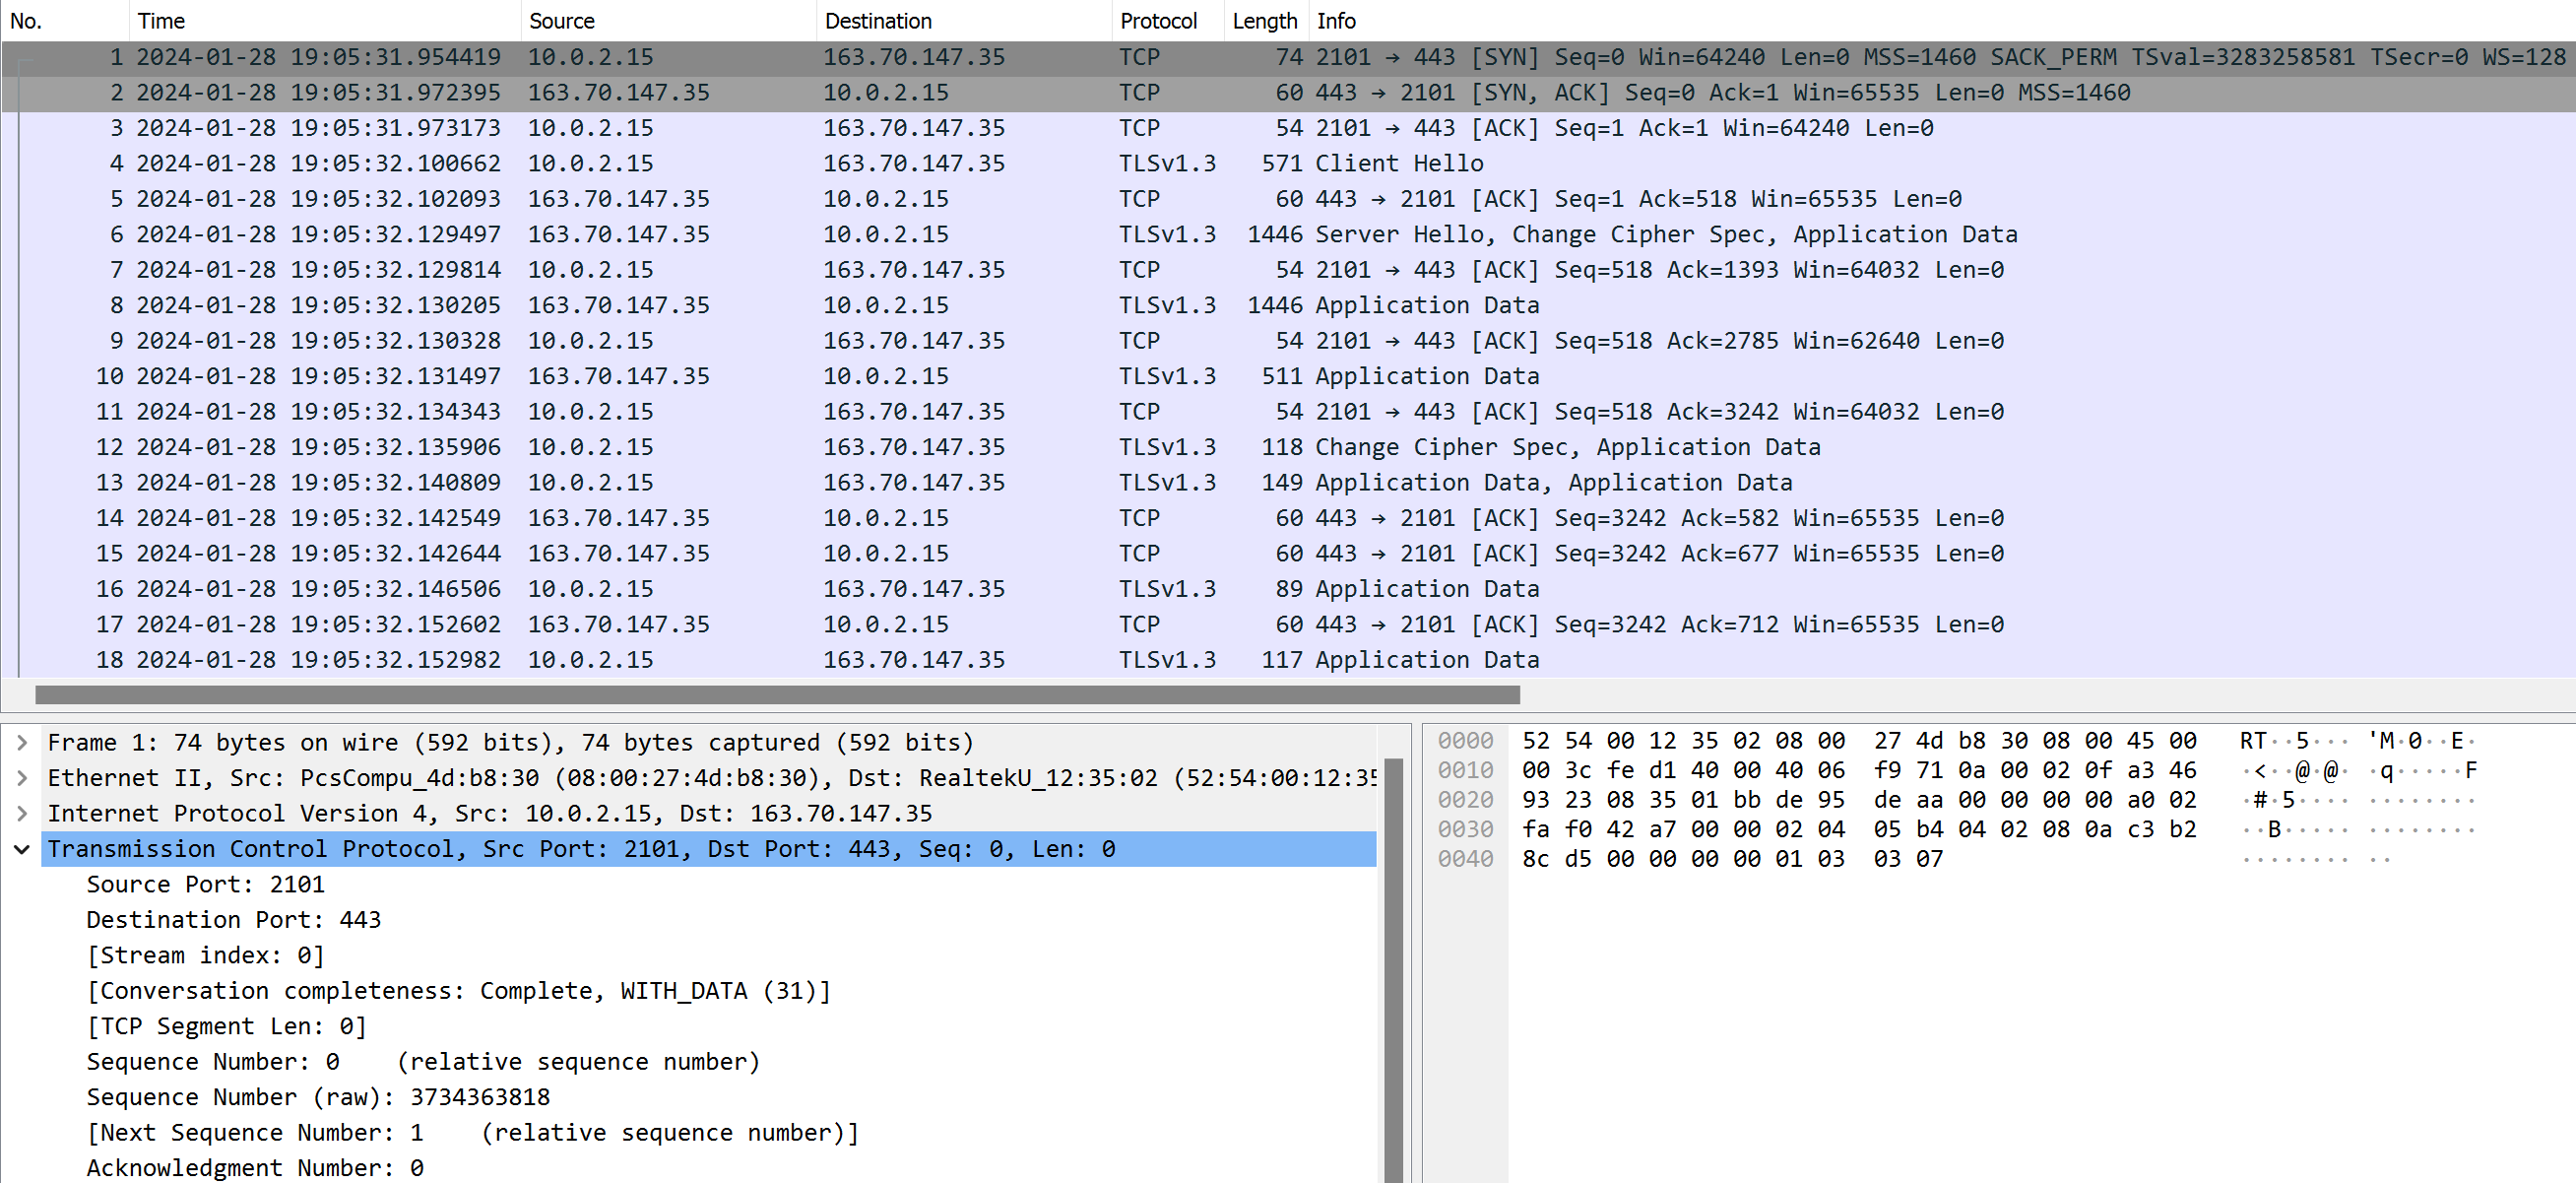
\includegraphics[width=1\linewidth]{images/wireshark.png}
    \caption{Sample \emph{pcap} file opened in Wireshark showing data extracted from the file generated after making a TCP connection to \emph{www.facebook.com} from Location 1.}
    \label{fig:pcapsample}
\end{figure}



\subsection{Calculating RTTs}

The RTT comparison between QUIC and TCP is an essential part of the data analysis of this experiment. Since the RTT of a certain connection is not preset, it must be calculated from the packet times for each connection instead. In order to calculate the RTT for a specific connection, TCP and QUIC vary in terms of what can be calculated.

\subsubsection{RTT for TCP Connections} In order to calculate the Average RTT for a TCP connection, RTTs for Server and Client needs to be calculated separately. The two average RTTs for Client and Server are calculated by finding the difference in time taken for a packet to be sent by the Client and received by the Server, and vice versa. After calculating the average RTT for the Server and Client, the average of these RTTs represents the total average RTT for the current connection.

\subsubsection{RTT for QUIC Connections} In QUIC connections, the same method for calculating RTT is not applicable because the packets are not necessarily sent or received in chronological order. Due to QUIC streams and multiplexing, a QUIC Client or Server is able to send and receive packets out of order, and re-order them afterwards. This makes an average RTT calculation more difficult, as the time between one packet being sent and it being received by the other endpoint could be longer or shorter than what it should be. In order to avoid this issue, calculating RTT for QUIC connections is possible by comparing acknowledgment numbers. The RTT for a specific packet will be the time difference between a packet with a certain number being sent, and the packet with the corresponding acknowledgement being received by the other endpoint. The total average RTT for a QUIC connection is calculated as the average of all the RTTs for each packet sent and received over the connection.


%==================================================================================================================================
\chapter{Results} 

This chapter aims to display and elaborate on the acquired data, including a discussion of these results. The data gathered represents all connection information regarding each URL queried, for both locations. This chapter includes information regarding connection establishment, time taken until data is transferred between the Client and Server, as well as information gathered about security, including the different TLS ciphers established and security errors that occurred during any connections.


In the results that follow, QUIC and TCP have been compared using percentages instead of site counts. This is due to the fact that there are much less sites able to support a QUIC connection compared to those able to support TCP. In order to fairly compare efficiency of connection establishment between the two transport protocols, percentages represent a clearer unit of measurement. Moreover, the graphs displayed include \emph{kernel density estimates}, which will be referred to as KDEs throughout this section.


\begin{table}[]
    \centering
    \caption{Percentage of connection attempts for QUIC vs TCP at each location. This table displays a count of how many connections were attempted, and how many out of these were either successful or failed for each location.}\label{tab:ConnectionAttempts}
    %\tt 
    \rowcolors{2}{}{gray!3}
    \begin{tabular}{lll|ll}
    \textbf{}     & \textbf{}  & \textbf{Connection Attempts} & \textbf{Successful} & \textbf{Failed} \\ \hline
    \textbf{QUIC} & \textbf{Location 1}     & 917          & 265                                & 652              \\
                  & \textbf{Location 2}    & 920          & 264                                & 656              \\
                  & \textbf{Total (\%)} &        & \textbf{28.8\%}                    & \textbf{71.2\%}  \\ \hline
    \textbf{TCP}  & \textbf{Location 1}    & 907     & 907                                & 0                \\
                  & \textbf{Location 2}     & 910     & 910                                & 0                \\
                  & \textbf{Total (\%)} &          & \textbf{100.0\%}                   & \textbf{0.0\%}  
    \end{tabular}
\end{table}


\section{Lack of Support for QUIC}

Table ~\ref{tab:ConnectionAttempts} shows the percentage of total sites for which a connection attempt was made, and comparing that to the total successful and failed connections for both transport protocols. It was found that around 30\% of the top 1000 sites support QUIC connections, whereas TCP is supported everywhere. Being a newly developed transport protocol, the support for QUIC connections across the world is bound to be limited. On the other hand, TCP has been in use for over forty years and is generally supported everywhere, which is clearly reflected in Table ~\ref{tab:ConnectionAttempts}. 

It is important to keep in mind, for the rest of the results discussed in this section, that QUIC was able to establish connections less than one third of all sites queried. This is significant because, when comparing this with TCP which has support all over the Internet, the data and results generated may display inconsistencies. However, with this in mind, all graphs and visualisations in this sections were adapted to display the results as accurately and fairly as possible.

\subsubsection{Limited Connection Attempts} As seen in Figure ~\ref{tab:ConnectionAttempts}, the number of connections attempted did not reach the full top 1000 URLs which were supposed to be queried in the experiment. There could be various reasons for this, which are explored in depth in the Evaluation section at the end of this Chapter. However, to properly analyse the results obtained for this experiment, it is important to keep in mind that not all queried URLs managed to establish a connection, and even less were able to support QUIC connections.

\section{Connection Establishment}

This section presents and discusses the obtained results relating to connection establishment. It was found generally that QUIC managed to establish connections faster than TCP at Location 1, while for Location 2 TCP proved to be the same if not slightly faster than QUIC in most cases. 

\subsection{Transport Handshake}

Figure ~\ref{fig:handshakeDuration} shows the duration of a transport handshake for both QUIC and TCP. From this visualisation, we can see that TCP's transport handshake has a slight overall advantage compared to the QUIC combined handshake: this is the case because, while the TCP has separate transport and security handshakes, QUIC has only one handshake which established both transport and security parameters \citep{Lang2017}. Therefore, although the TCP transport handshakes have a shorter duration compared to QUIC's, they also lack any form of security and encryption at this point. 

At Location 1, the maximum of the QUIC KDE is at around 60ms, whereas for TCP  it is at around 25ms. This indicates that TCP is more than twice as fast as QUIC when it comes to  connection establishment. 

For Location 2, this difference is even more evident. With TCP's KDE at arouns 15ms and QUIC's at around 40ms, TCP is once again showing a faster connection-establishment time compared to QUIC. 

Despite the results shown in Figure ~\ref{fig:handshakeDuration}, this visualisation is not representative of the entire connection establishment process. This figure ignores any security parameters, only revealing the time taken to establish a connection. At this point only the QUIC handshakes have established security parameters, whereas the TLS handshake still needs to occur in TCP connections.\\

\begin{figure}[hbtp]
    \centering
    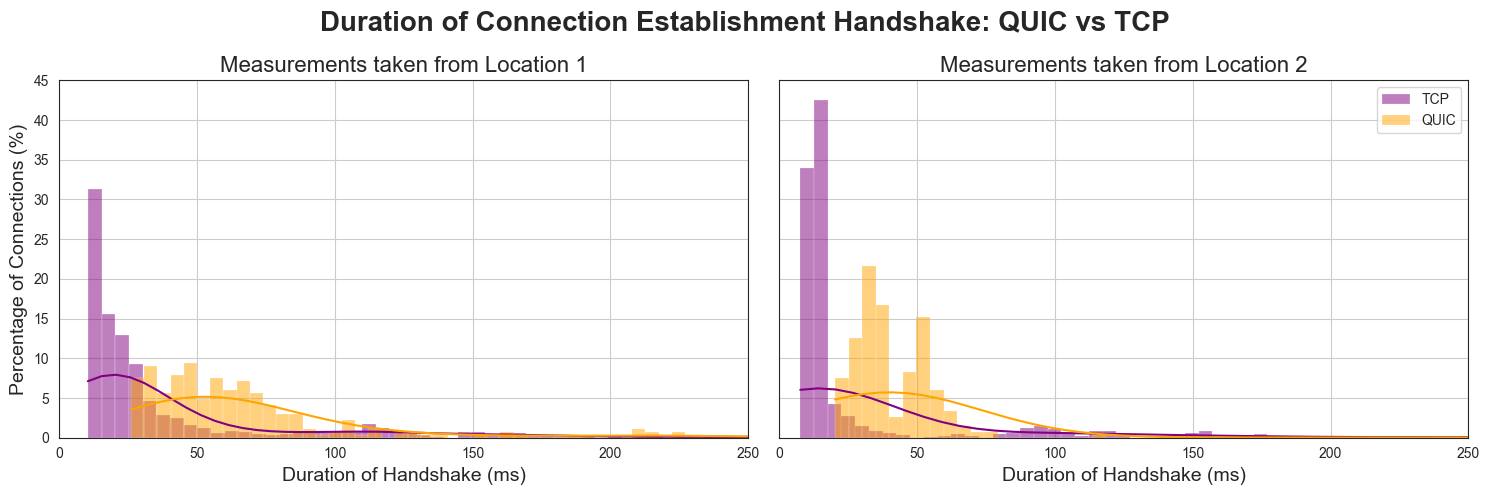
\includegraphics[width=1\linewidth]{images/connectionEstablishment.png}
    \caption{These histograms depict the time taken to establish a connection via a transport handshake with a specified URL, comparing the QUIC and TCP transport protocols. The plot on the left shows data collected from Location 1, while the one on the right shows data collected from Location 2. The graphs include kernel density estimates for easier visualisation.}
    \label{fig:handshakeDuration}
\end{figure}

However, it is still worth noting that, despite not having any security parameters, TCP is faster at establishing connections compared to QUIC. While most TCP connections are established after around 10ms, QUIC connections need at least 20-25ms. Additionally, TCP connections require less time overall to establish than QUIC connections, as the distributions show much higher percentages for the faster connection establishment times in TCP than for QUIC.


\subsection{Comparing Transport and Security Handshakes}


QUIC relies on a combined handshake to minimize latency during connection establishment by using a 1-RTT handshake that establishes both transport and security parameters in only one round trip \citep{Lang2017, Thom2020}. This is apparent in Figure ~\ref{fig:CEvsTLS_QUIC}, where the end of the connection establishment handshakes happen almost at the exact same time as the end of the TLS handshake, clearly depicting a combined handshake. Moreover, the distribution of data in the various bins is also almost identical for both handshakes.


On the other hand, TCP has separate connection establishment and security handshakes. Figure ~\ref{fig:CEvsTLS_TCP} clearly depicts this aspect of establishing a secure connection with TCP. 

In Figure ~\ref{fig:CEvsTLS_TCP}, the distribution of the three-way handshake for the data obtained at Location 1 clearly occurs before the TLS handshake. The duration of the three-way handshake is around 25ms and, while the peak of the KDE for the TLS handshake data is less significant and occurs roughly 60-80ms afterwards. Due to the TLS handshake data not having a clear maximum in its KDE, the TLS handshake is not necessarily occurring immediately after connection establishment. In the following subsection, this will be explored in more detail.

For Location 2, the distinction between the three-way handshake and the TLS handshake is clearer. These distributions have maxima which are roughly 60ms apart, indicating that the two handshakes are occurring sequentially. As well as the clear distinction between the two handshakes, the distribution of the TLS handshake duration for Location 2 in Figure ~\ref{fig:CEvsTLS_TCP} has a significant feature: there is a small peak in the TLS handshake distribution that occurs at the same time as the three-way handshake. There are different TCP features which could cause this to happen, but it is unknown from the results of this experiment what exactly has caused this occurrence.

\subsubsection{TCP Fast Open (TFO)} One possible explanation for the peak in the distribution of the TLS handshake for Location 2 in Figure ~\ref{fig:CEvsTLS_TCP} is TCP Fast Open (TFO). TFO allows the Client to send the TLS ClientHello message in the SYN packet of a TCP connection, which reduces the number of round trips required to establish a new connection and send data. \citet{Cheng2014} state that "For Transport Layer Security (TLS) over TCP, it is safe and useful to include a TLS client\_hello in the SYN packet to save one RTT in the TLS handshake." \citep{Cheng2014}. This could lead to the three-way handshake and TLS handshake ending at the same time. Additionally, it makes sense that this would only occur at Location 2, given that the server at that location is faster and more powerful than the one at Location 1.


\begin{figure}
    \centering
    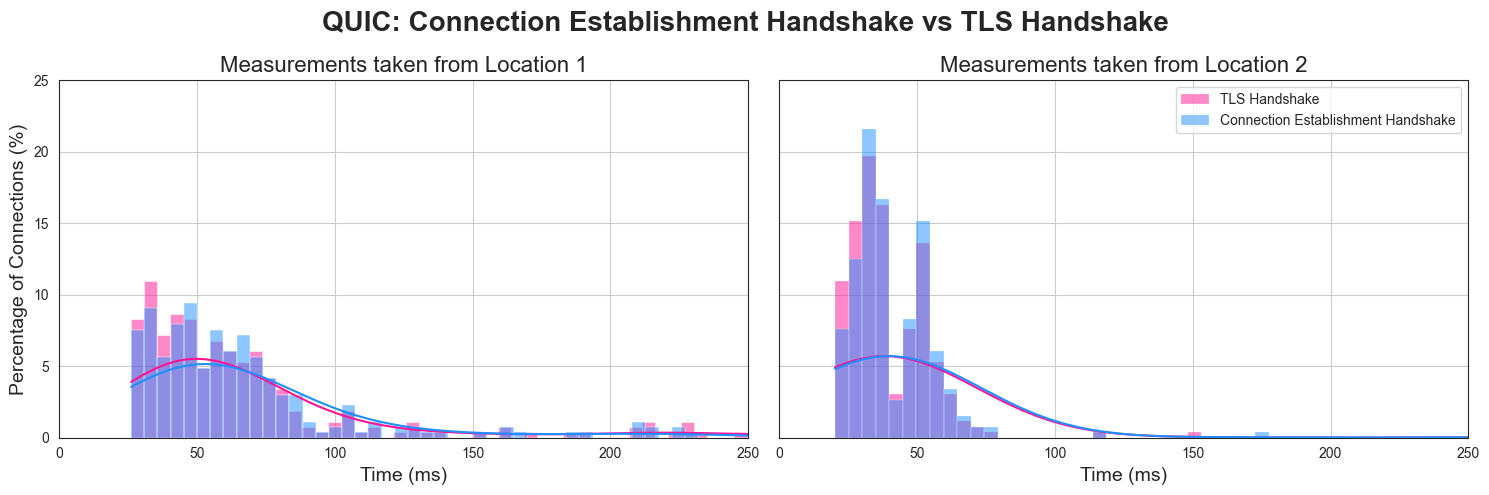
\includegraphics[width=1\linewidth]{images/transport_security_handshakes_QUIC.png}
    \caption{These histograms show the time taken to finish a Connection Establishment handshake vs a TLS handshake using QUIC.}
    \label{fig:CEvsTLS_QUIC}
\end{figure}


\begin{figure}
    \centering
    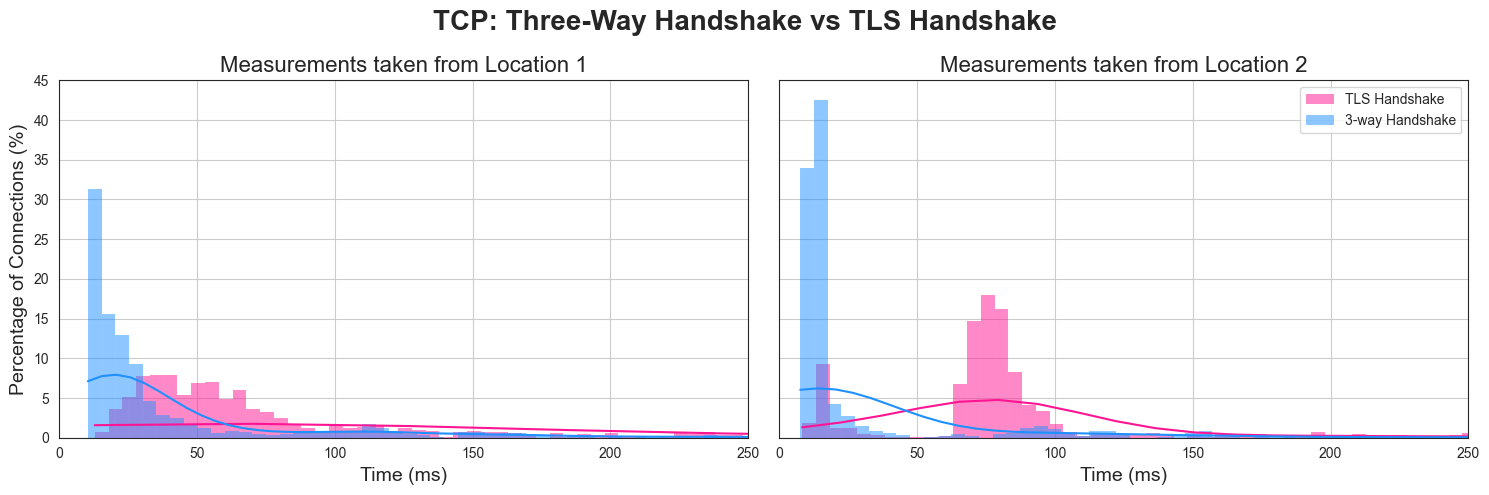
\includegraphics[width=1\linewidth]{images/transport_security_handshakes_TCP.png}
    \caption{These histograms show the time taken to finish a Connection Establishment handshake vs a TLS handshake using TCP.}
    \label{fig:CEvsTLS_TCP}
\end{figure}

\subsection{Delay of TLS Handshake with TCP in Location 2}

In Figure ~\ref{fig:CEvsTLS_TCP}, the leftmost graph shows the TLS handshake data not having a clear maximum in its KDE. This implies that the TLS handshake is not necessarily occurring immediately after connection establishment. 

A delay in the completion of the TLS handshake could be due to various factors. One possible cause for this behaviour could be that the application we are connecting to may require the Client or Server to initialise certain application-layer protocols, such as HTTP, before starting the TLS handshake. This could include the negotiation of protocol-specific parameters, exchanging application-layer data, or performing other setup tasks. 

Another possible explanation could be that the server may need time to retrieve and configure the appropriate TLS certificate, select the appropriate encryption algorithms and parameters, and perform other initialization tasks required for the TLS handshake before actually executing it. 

Moreover, the TLS handshake also involves several round trips between the Client and Server in order to negotiate encryption parameters, exchange cryptographic keys, and verify certificates. This handshake process can introduce additional latency compared to the three-way handshake, which can affect the overall connection establishment time and thus the time at which the TLS handshake is complete.

Finally, another reason for the TLS handshake to be delayed could be due to connection reuse. In scenarios where TCP connection reuse is enabled, the Server may decide to reuse an existing TCP connection for subsequent requests by creating a Transmission Control Block (TCB) to manage the connection state. If the Server caches TCB states for recently closed connections, it can potentially reuse an existing TCB for subsequent connections from the same Client \citep{Egge2000}. However, if the server's resources are limited or if the TCB cache becomes too large, it may delay the allocation of resources required for processing incoming TLS handshake requests, potentially leading to increased TLS handshake latency.

\section{Time Before Data Transfer}

\begin{figure}
    \centering
    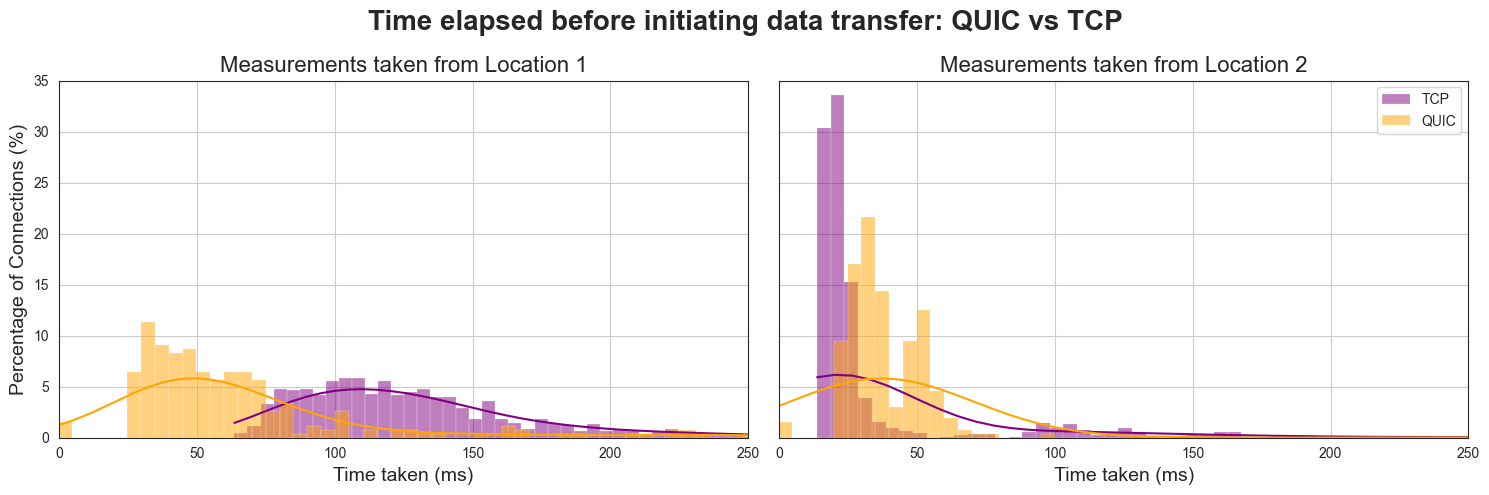
\includegraphics[width=1\linewidth]{images/time_to_data_transfer.png}
    \caption{These histograms depict the time taken before data is transferred in a Client-Server connection for each of the queried URLs, split into the data from both locations. The plot on the left shows data collected from Location 1, whereas the one on the right shows data collected from Location 2.}
    \label{fig:timeBeforeDataTransfer}
\end{figure}


Figure ~\ref{fig:timeBeforeDataTransfer} shows the time taken to establish a connection with a specified URL, using both QUIC and TCP. From this visualisation, it is unclear whether QUIC is actually faster than TCP. 

When establishing a connection from Location 1, QUIC seems to take less time to establish a connection and transfer data compared to TCP: the maximum for the QUIC KDE is at around 50ms, while that of the TCP KDE is at around 110ms. This would make QUIC more than twice as fast at establishing a connection with a server and transferring data compared to TCP. 
Moreover, the maxima of the two KDEs in this graph both show that around 5\% of all connections were established at their maximum point. Additionally, most other connections were established symmetrically at this point, indicating that the two sets of data are normally distributed, where the mean time to data transfer is 40ms for QUIC and 110ms for TCP, and the standard deviation is the size of the bins, which is 5ms.

Based on the data collected at Location 2, it is not very clear whether QUIC is actually faster than TCP at establishing a connection. In the graph for measurements taken at Location 2, the peak for time before data transfer with TCP is at around 25ms, whereas that of QUIC is at around 40-45ms: this would make TCP roughly 40\% faster than QUIC at transferring data at this location. Moreover, the majority of connections established with TCP (almost 35\%) were able to transfer data in 25ms or less, while most of the QUIC connections (just over 20\%) were established in around 40ms. This would make QUIC almost two times slower than TCP at this location.

However, it is important to notice that the KDE for QUIC connections is very similar in both graphs. This indicates that QUIC is perhaps more consistent in its behaviour compared to TCP. The inconsistency in time taken to establish a connection with TCP can be caused by various factors depending on the location from which TCP is trying to connect, such as network congestion, firewalls, or load balancing in the network.

\subsection{Difference in Time Taken}

\begin{figure}
    \centering
    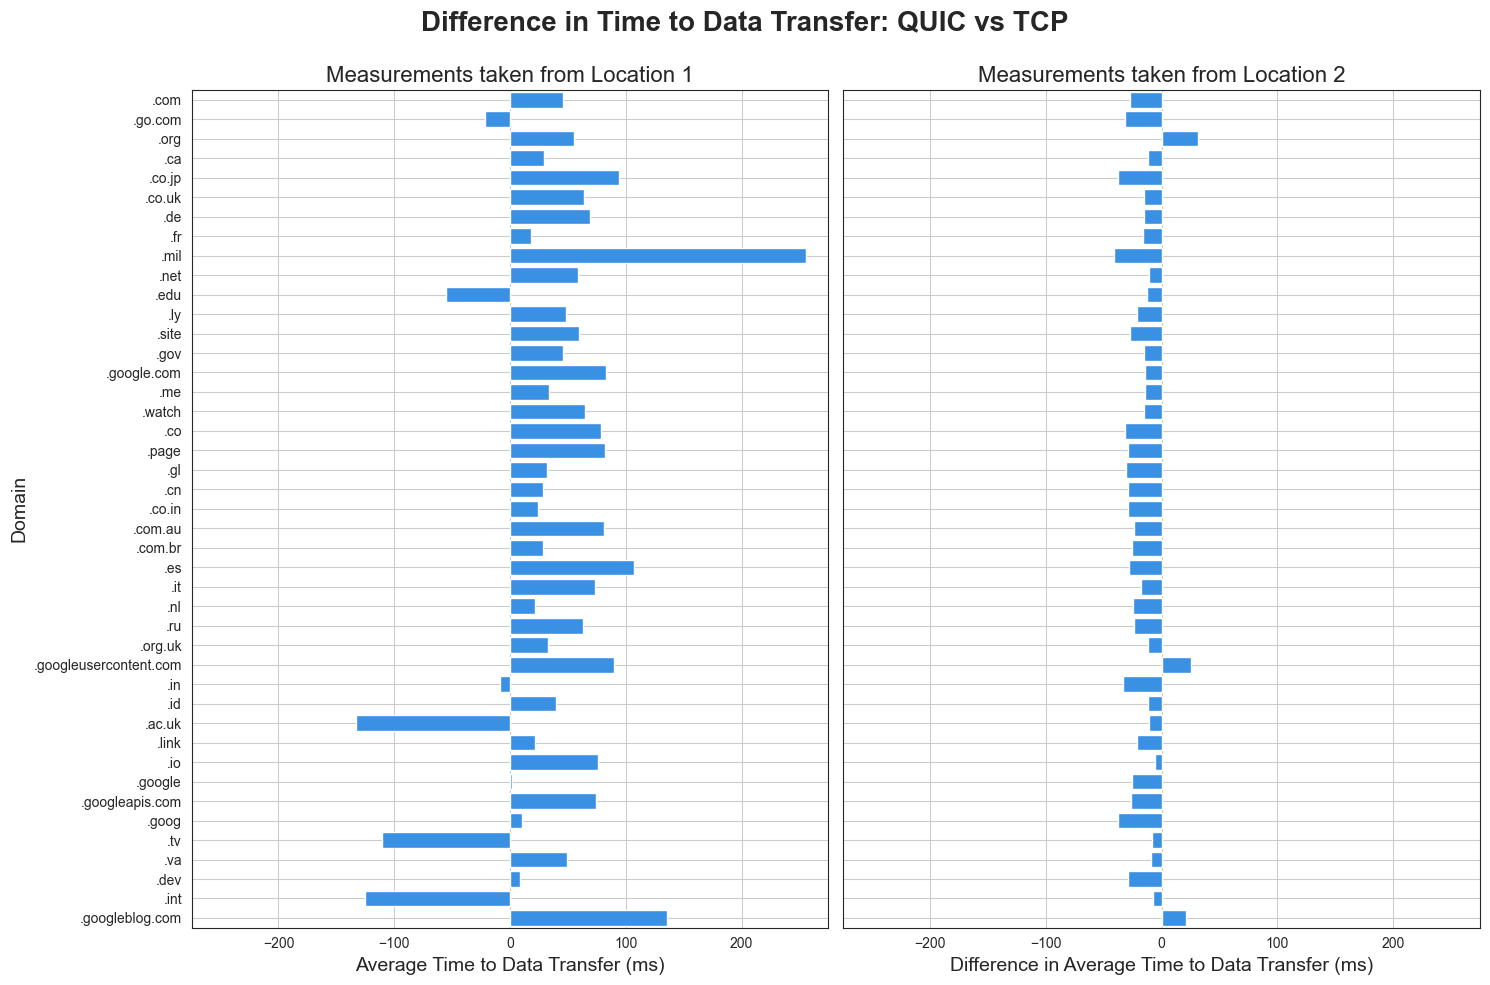
\includegraphics[width=1\linewidth]{images/domainDifference_QUICvsTCP.png}
    \caption{These graphs show the average difference in time taken to establish a connection and transfer the first byte of data for each URL in a certain domain. A positive value indicates that QUIC connections were faster, whereas a negative value indicate TCP was faster.}
    \label{fig:domainDifference}
\end{figure}

Figure ~\ref{fig:domainDifference} displays an average of the difference in time taken before initiating data transfer between QUIC and TCP connections for each queried URL in a certain domain. It is clear from this visualisation that QUIC is much faster than TCP from Location 1, whereas from Location 2 QUIC seems to be slightly slower than TCP. 

Aside from a few outliers, QUIC connections were generally between 50-100ms faster than TCP connections at reaching the data transfer stage at Location 1. This indicates that, from a home router, QUIC tends to perform better and establish connections more quickly than TCP.

On the other hand, at Location 2 it seems as though TCP was slightly faster than QUIC throughout every queried domain. This implies that high-speed servers are able to establish initial parameters and perform the TCP and TLS handshakes faster than they can perform the combined handshake for QUIC connections.

Overall, QUIC connections were generally found to be faster than TCP connections. However, when querying sites from a high-speed router, TCP might still have the upper hand.

Although Figure ~\ref{fig:domainDifference} is clear in displaying the general trend for the difference in the time before data transfer between QUIC and TCP, it only shows an average of time differences for each domain. In order to properly visualise the entire dataset, the Appendices ~\ref{fig:urlDifference_p1}, ~\ref{fig:urlDifference_p2}, ~\ref{fig:urlDifference_p3}, and ~\ref{fig:urlDifference_p4} represent a further visualisation of the time before data transfer, by displaying the difference in the time taken to send the first data packet in a connection for each individual URL. Other than a few outliers, it is quite clear from these visualisations as well that QUIC tends to be faster at establishing a connection and proceeding with data transfer than TCP is. However, the data collected at Location 2 seems to show TCP take the same amount of time if not slightly less than QUIC to establish connections and transfer the first data packet, whereas QUIC tends to have a greater advantage in speed compared to TCP at Location 1.


\section{Round Trip Time}


\begin{figure}
    \centering
    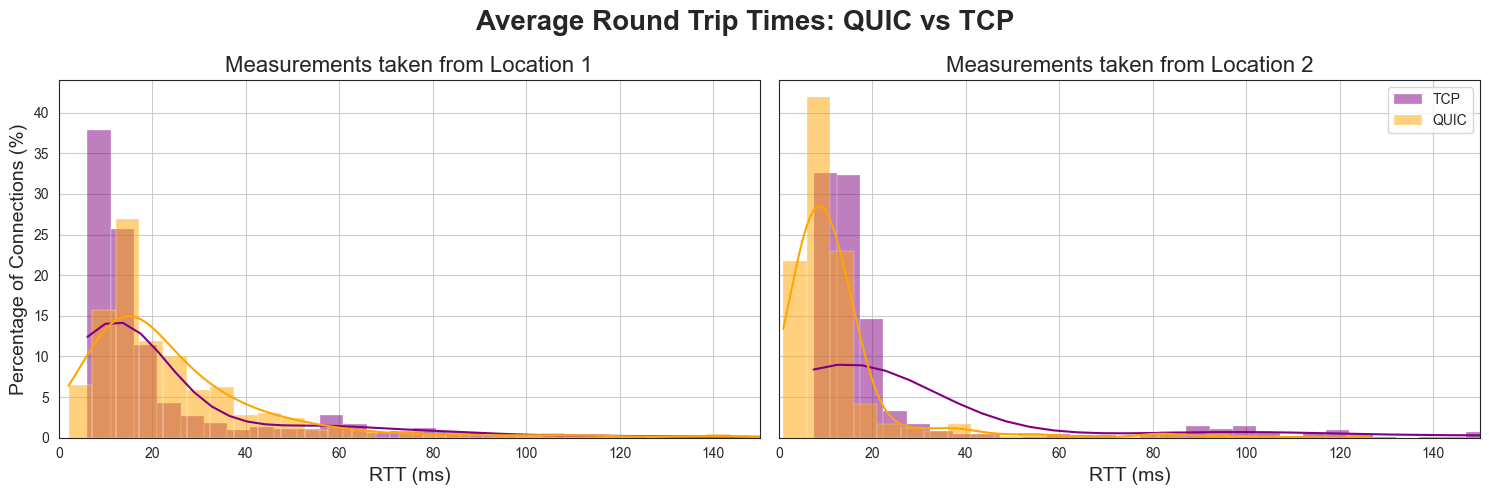
\includegraphics[width=1\linewidth]{images/RTTs.png}
    \caption{These histograms depict the percentage of observed connections with a certain average round trip time, split for each location. The plot on the left shows data collected from Location 1, whereas the one on the right shows data collected from Location 2.}
    \label{fig:RTTs}
\end{figure}

Figure ~\ref{fig:RTTs} shows the RTTs for QUIC and TCP. This visualisation shows that, from Location 1, the average round trip times for both QUIC and TCP are roughly the same. For Location 2 on the other hand, QUIC seems to have a clear upper hand in terms of RTT.

Observing the leftmost set of axes, we notice that the maxima for the KDEs of both QUIC and TCP connections are almost at the same point. For QUIC connections, the majority (15\%) had an average RTT of 15ms, and around 14\% of TCP connections had an average RTT of roughly 12-13ms. Despite the KDEs being very similar for the two transport protocols, observing the connections with RTTs of under 10ms, we notice from this graph that more TCP connections have an extremely fast RTT than QUIC connections do. almost 40\% of TCP connections had an RTT between 5-10ms, while only 15\% of QUIC connections had the same RTT. 

This is inconsistent with our knowledge of the QUIC transport protocol, which has been designed especially to reduce latency and reduce overall round trip times for its connections. However, the actual RTT experienced by TCP and QUIC connections can vary depending on factors such as network congestion, packet loss, server and client implementations, and the specific characteristics of the network environment. The behaviour of TCP and QUIC exhibited while connecting to sites from Location 1 could have been affected by one or more of the aforementioned factors.

Despite that, it is also important to note that, while no TCP connection had an RTT of under 5ms, around 6\% of QUIC connections did. Additionally, TCP connections had a lot more RTTs of 50ms or more compared to QUIC connections.

The histogram representing the data retrieved at Location 2 is very different from the data at Location 1. In this graph, it is clear that QUIC really has a much shorter RTT compared to TCP. Over 40\% of QUIC connections had an RTT of 5-10ms, and around 22\% had an RTT of 0-5ms. This shows that over 60\% of all QUIC connections have an RTT of under 10ms. If we count the next RTT bin of connections with a RTT of 10-15ms, that gives an additional 13\%, meaning that around 75\% of all QUIC connections have an RTT of up to 15ms.

The TCP connections established at Location 2 have a maximum KDE at around 10\% of connections with a RTT of 15-20ms. Moreover, none of the TCP connections had an RTT of under 5ms: compared to QUIC's 22\%, this really shows the difference between the two transport protocols. However, although QUIC has an average RTT which is much shorter than that of TCP at this location, this graph also shows that almost no TCP connections have an RTT of above 25ms. 

In general, QUIC has a much shorter RTT compared to TCP. This is due to many features that QUIC has implemented, such as the use of concurrent streams, independent packet delivery and packet reordering, which allow this new transport protocol to exhibit much lower RTTs compared to TCP.


\section{TLS Cipher Suites}

This section will elaborate on the establishment of TLS Cipher Suites in both QUIC and TCP connections. Overall, it was found that both QUIC and TCP managed to establish TLS Cipher Suites for the vast majority of the established connections. Although TCP demonstrated more variation in the authentivation and key exchange algorithms used, QUIC proved to be extremely efficient in establishing TLS ciphers, indicating that QUIC is more than able to establish secure parameters in its connections. However, it was also found that TLS-related error messages were much more frequent in QUIC connections compared to TCP ones.


\subsection{TLS Cipher Suites established in QUIC Connections}

\begin{table}[hbtp]
    \centering
    \caption{The TLS Ciphers found when analysing all QUIC connections, along with the number of sites found using each cipher.}\label{tab:TLSCiphers_QUIC}
    %\tt 
    \rowcolors{2}{}{gray!3}
    \begin{tabular}{lll|l}
    \textbf{TLS Ciphers established in QUIC Connections}                                & \multicolumn{2}{c|}{\textbf{No. of sites}}  & \textbf{Total} \\ 
    \textbf{}                                           & \textbf{Location 1} & \textbf{Location 2}         \\ \hline %\midrule % optional rule for header 
    AES256\_GCM          & 70                  & 70                  & 140            \\
    AES128\_GCM          & 191                 & 190                 & 381            \\ \hline
                         & 260                 & 260                 & \textbf{521}  
    \end{tabular}
\end{table}


In order to analyse the results in this section correctly, it is important to keep in mind that only 529 QUIC connections were established successfully during this experiment. Examining Table ~\ref{tab:TLSCiphers_QUIC}, we can observe that around 98\% of all QUIC connections established were able to provide a TLS cipher. This is a very high number of connections, which indicates that the vast majority of QUIC connections were secure and encrypted.

Regarding the individual ciphers, QUIC connections do not display a wide variety of choices: all ciphers found were representative of only two distinct TLS ciphers. Table ~\ref{tab:TLSCiphers_QUIC} shows that around 73\% of QUIC connections were found to be using the AES128\_GCM cipher, and around 27\% were using AES256\_GCM. While AES256 theoretically provides a higher level of security than AES128 as it uses a larger key for encryption and decryption, AES128 is still considered secure against all known practical attacks. AES128\_GCM also provides both encryption and authentication, ensuring confidentiality and integrity of the transmitted data.


\subsection{TLS Cipher Suites established in TCP Connections}

TCP connections were very successful at establishing TLS cipher suites: over 90\% of all connections were able to establish one of the cipher suites seen in Table ~\ref{tab:TLSCiphers_TCP}. This is more significant compared to the QUIC connections because the packet capture script was able to connect to many more sites using TCP as opposed to QUIC. Therefore, the dataset available for TCP connections was a lot bigger in this experiment.

The majority of TCP connections (around 80\%) established either an AES\_256\_GCM cipher with SHA384, or AES\_128\_GCM cipher with SHA256. By combining AES256 encryption with SHA384 hashing, TLS cipher suites can achieve a higher level of robustness and security. AES256 provides strong confidentiality for encrypted data, while SHA384 ensures the integrity and authenticity of the data by generating a secure hash value. The same is true for AES128 and SHA256, except slightly less secure due to the reduced key length.

The following group of popular TLS cipher suites established in TCP connections is the ones using an ECDHE key exchange algorithm in combination with RSA, used in around 15\% of TCP connections. Both ECDHE and RSA offer strong security properties for key exchange: ECDHE provides forward secrecy, while RSA enables authentication and verification of digital signatures. By using both algorithms together, TLS connections benefit from both forward secrecy and strong authentication, enhancing security and trust in the communication. This is a particularly good combination, because while ECDHE offers forward secrecy and strong security, it may not be supported by every Client or Server. On the other hand, RSA is widely supported and can be used as a fallback option for key exchange in cases where ECDHE is not available or practical: this ensures compatibility with a broader range of systems and devices.

Another fairly common combination among TLS cipher suites in TCP connections is ChaCha20 used alongside Poly1305, used in roughly 7-8\% of all TCP connections. When used together, ChaCha20 and Poly1305 offer excellent performance for both encryption and authentication. They can provide fast and secure communication with minimal computational overhead, making them ideal for real-time applications and high-speed networks.


\begin{table}[hbtp]
    \centering
    \footnotesize
    \caption{The TLS Ciphers found when analysing all TCP connections. As shown, not all sites were able to establish a TLS Cipher: there were 27 URLs with missing ciphers from location 1 and 19 missing from location 2.}\label{tab:TLSCiphers_TCP}
    %\tt 
    \rowcolors{2}{}{gray!3}
    \begin{tabular}{lll|l}
    %\toprule
    \textbf{TLS Cipher Suites established in TCP Connections}                                & \multicolumn{2}{c|}{\textbf{No. of sites}}  & \textbf{Total} \\ 
    \textbf{}                                           & \textbf{Location 1} & \textbf{Location 2}        \\ \hline %\midrule  
    TLS\_AES\_256\_GCM\_SHA384                          & 493           & 484             & 977            \\
    TLS\_ECDHE\_RSA\_WITH\_AES\_128\_GCM\_SHA256        & 55            & 56              & 111            \\
    TLS\_AES\_128\_GCM\_SHA256                          & 217           & 230             & 447            \\
    TLS\_DHE\_RSA\_WITH\_AES\_256\_GCM\_SHA384          & 1             & 1               & 2              \\
    TLS\_ECDHE\_ECDSA\_WITH\_AES\_256\_GCM\_SHA384      & 2             & 2               & 4              \\
    TLS\_ECDHE\_ECDSA\_WITH\_AES\_128\_GCM\_SHA256      & 9             & 9               & 18             \\
    TLS\_ECDHE\_RSA\_WITH\_CHACHA20\_POLY1305\_SHA256   & 52            & 52              & 104            \\
    TLS\_ECDHE\_RSA\_WITH\_AES\_256\_GCM\_SHA384        & 42            & 39              & 81             \\
    TLS\_ECDHE\_ECDSA\_WITH\_CHACHA20\_POLY1305\_SHA256 & 9             & 9               & 18             \\
    TLS\_CHACHA20\_POLY1305\_SHA256                     & 10            & 10              & 20             \\ \hline
                                                        & 890           & 901             & \textbf{1782} 
    \end{tabular}
\end{table}


\section{TLS Alerts}

In this section, the frequency and nature of TLS Alerts and TLS-related connection errors will be investigated. It was found that, TLS-related error messages were roughly six times more frequent in QUIC connections than in TCP connections. 

\subsection{TLS Alerts in QUIC Connections}


\begin{table}[hbtp]
    \caption{The connection errors found when analysing all QUIC connections, along with a count of how many connections encountered each error at both locations.}\label{tab:TLSErrors_QUIC}
    \centering
    %\tt 
    \rowcolors{2}{}{gray!3}
    \begin{tabular}{p{7cm}p{2cm}p{2cm}|p{1cm}}
    %\toprule
    \textbf{Connection Errors found with QUIC}                              & \multicolumn{2}{c}{\textbf{No. of errors}}  & \textbf{Total} \\ 
    \textbf{}                                           & \textbf{Location 1} & \textbf{Location 2}         \\ \hline %\midrule % optional rule for 
    kthxbye                                                                                   & 257           & 256 & 513             \\ 
    200:TLS handshake failure (ENCRYPTION\_INITIAL) 80: internal error                        & 155           & 148 & 303            \\
    handshake failed                                                                          & 2             & 3   & 5              \\
    28:Reject connection                                                                      & 2             & 2   & 4              \\
    TLS Alert 80                                                                              & 1             & 2   & 3              \\
    28:TLS handshake failure (ENCRYPTION\_INITIAL) 40: handshake failure                      & 2             & 2   & 4              \\
    cannot decrypt token                                                                      & 0             & 2   & 2              \\ \hline
    \textbf{Total Connection Errors}                                                          & 419           & 415 & \textbf{834}   \\ 
    \textbf{Total TLS-related Errors}                                                         & 158           & 152 & \textbf{310}  
    \end{tabular}
\end{table}



Given that \emph{qlog} files do not have a TLS-specific error category, it is only possible to observe TLS errors within the "connection errors" field. Table ~\ref{tab:TLSErrors_QUIC} shows the number of connection errors which occurred for all URLs at each location, and displays a total count of only TLS-related errors on the bottom row.

\subsubsection{internal\_error} The TLS alert found in QUIC connections that represents the most significant TLS-related connection error is the internal\_error alert with code 80. Despite having different error messages, this alert is probably the same in the second and fifth lines of Table ~\ref{tab:TLSErrors_QUIC}. This TLS alert is described in the TLSv1.3 specification as follows.

\begin{quote}
    An internal error unrelated to the peer or the correctness of the protocol makes it impossible to continue, such as a memory allocation failure. The error is not related to protocol. This message is always fatal. 
    \citep{Resc2018}
\end{quote} 

When a TLS internal\_error alert is received, it indicates that something unexpected has occurred within the TLS endpoint's internal logic or processing. This alert might be due to incompatibility issues among TLS implementations in both the Client and Server.


\subsubsection{handshake\_failure} The only other error which has evidently to do with TLS is the one on the sixth line of Table ~\ref{tab:TLSErrors_QUIC}. This is the handshake\_failure alert with code 40 and is described in the TLSv1.3 specification as follows.

\begin{quote}
    Reception of a handshake\_failure alert message indicates that the sender was unable to negotiate an acceptable set of security parameters given the options available. This is a fatal error.
    \citep{Resc2018}
\end{quote}

This alert indicates that something went wrong while trying to establish security parameters during the TLS handshake, and the entire connection had to be aborted.

\subsubsection{decrypt\_error} The final error listed in Table ~\ref{tab:TLSErrors_QUIC} could represent the decrypt\_error token with alert code 51, which would indicate that the connections during which this error occurred were "unable to correctly verify a signature or validate a TLS Finished message" \citep{Resc2018}.


\subsection{TLS Alerts in TCP Connections}


\begin{table}[hbtp]
    \centering
    \caption{The TLS-related errors found when analysing all TCP connections, along with their Alert descriptions as specified in \citet{Resc2018}. The lowest row represents all errors caught for which there was no available description, as the data was encrypted.}\label{tab:TLSErrors_TCP}
    %\tt 
    \rowcolors{2}{}{gray!3}
    \begin{tabular}{lll|l}
    %\toprule
    \textbf{TLS Alerts found in TCP Connections}                                & \multicolumn{2}{c|}{\textbf{No. of errors}}  & \textbf{Total} \\ 
    \textbf{}                                           & \textbf{Location 1} & \textbf{Location 2}         \\ \hline %\midrule % optional rule for header 
    20:bad\_record\_mac                   & 0                   & 1                   & 1              \\
    41:no\_certificate\_RESERVED           & 1                   & 0                   & 1              \\
    50:decode\_error                       & 1                   & 0                   & 1              \\
    70:protocol\_version                  & 1                   & 0                   & 1              \\
    115:unknown\_psk\_identity            & 1                   & 0                   & 1              \\
    255:unsupported\_extension            & 0                   & 1                   & 1              \\
    Encrypted Error Message                & 32                  & 12                  & 44             \\ \hline
                                           & 36                  & 14                  & \textbf{50}   
    \end{tabular}
\end{table}


Most TLS alert messages were encrypted in the TCP connections, and therefore the majority of error messages found and displayed in Table ~\ref{tab:TLSErrors_TCP} are impossible to understand. This is because, after the TLS handshake has been completed, the header and payload of every following packet will be encrypted using the established TLS cipher suite. However, it was possible to see that certain errors occurred before connection establishment was complete, and we can observe which errors occurred at which location. 

\subsubsection{no\_certificate\_RESERVED} The no\_certificate\_RESERVED alert with code 41 was used in SSLv3 but not any version of TLS. \citet{Resc2018} states that this alert cannot be sent by TLS implementations, so perhaps this can be treated as an internal error or another issue to do with compliance to certain TLS policies. 

\subsubsection{unknown\_psk\_identity} The alert with code 115 unknown\_psk\_identity is not mentioned in the TLSv1.2 or 1.3 RFC specifications, however, \citet{Tscho2005} presented a standard for supporting TLS authentication based on pre-shared keys and stated the following.

\begin{quote}
    If the server does not recognize the PSK identity, it MAY respond with an "unknown\_psk\_identity" alert message.  Alternatively, if the server wishes to hide the fact that the PSK identity was not known, it MAY continue the protocol as if the PSK identity existed but the key was incorrect: that is, respond with a "decrypt\_error" alert. \citep{Tscho2005}
\end{quote}

Therefore, in one instance at Location 1, the Server was unable to recognise the identity of the pre-shared key used for authentication.

\subsubsection{decode\_error and protocol\_version} The alert decode\_error with code 50 indicates that a field was out of the specified range or that the length of the message was incorrect, while the protocol\_version alert with code 70 indicates that during the connection there was an attempt at negotiating a protocol version which is not supported by TLS. These alerts were both generated during TCP connections at Location 1.

\subsubsection{bad\_decode\_mac and unsupported\_extension} The alert bad\_decode\_mac with code 20 indicates that an incorrect message authentication code was used during connection establishment. The unsupported\_extension alert with code 255 indicates that the Client the extension received within a ServerHello did not correspond to the one the Client places in the corresponding ClientHello. These alerts were both generated during TCP connections at Location 2.


\section{Evaluation}

Overall, the results gathered from the data collection script produced very detailed and accurate visualisations which are coherent with what we know about the QUIC and TCP transport protocols. This experiment managed to take accurate measurements through the use of multi-threading and using different source ports for each queried site. Moreover, the top 1000 URLs list used was up to date at the time of the experiment. 

In this section, the results presented in this chapter will be compared to this project's related work. Any limitations observed in this measurement study will be discussed below.

\subsection{Comparison with Related Work}

\subsubsection{QUIC vs TCP} In general, the results obtained from this experiment align with those from similar studies. \citet{Kakh2017} found similar results when comparing QUIC and TCP performance, concluding that QUIC does generally perform better than TCP in most cases. \citet{Grat2016} also showed an extremely similar outcome, as TCP was found to perform better than QUIC in networks with high latency and low bandwidth: this can be seen in Figure ~\ref{fig:timeBeforeDataTransfer} where TCP is shown to perform better than QUIC at Location 2.

\subsubsection{QUIC Performance \& Security} The overall performance and security of QUIC connections found in the results of this experiment are in line with the expectations for the transport protocol. QUIC connections were mostly encrypted using AES, and the combined transport and cryptographic handshake proved to be efficient in establishing TLS ciphers for secure connections, indicating that QUIC is more than able to establish security parameters in its connections. However, it was also found that TLS-related error messages were roughly six times more frequent in QUIC connections compared to TCP ones. Despite that, QUIC did show a significant improvement in speed compared to TCP in most aspects of connection establishment and RTT, as seen in Figures ~\ref{fig:handshakeDuration}, ~\ref{fig:timeBeforeDataTransfer}, ~\ref{fig:domainDifference} and ~\ref{fig:RTTs}.

\subsection{Limitations}

\subsubsection{Missing Measurements} Due to unforeseen issues encountered at the different locations, there is a small amount of missing data. More specifically, only 917 URLs were queried successfully with QUIC and 907 with TCP from Location 1, while from Location 2 only 920 URLs were queries with QUIC and 910 with TCP. Despite still being a very high number, it is unsure why the remaining URLs failed to generate any data. This could be due to various issues relating to the state of the network environment in which the sites were queried, as well as the condition of the virtual machine from which the packet capture script was run. For instance, while capturing packets using tools like \emph{tcpdump}, there might be cases where packets are dropped or not captured properly: this could lead to missed connections or incomplete data, which could have affected the total number of successful queries. 
Another possible explanation could be that the Linux VM or the network environment in which it was operating could have firewall rules or network configurations that restrict certain types of connections, or impose limitations on the number of concurrent connections occurring at a certain middlebox. 
Additionally, the Linux VM or the underlying infrastructure might have resource limitations such as bandwidth constraints, connection limits, or CPU/memory constraints that impact both QUIC and TCP connections: if the system reaches its limits, it can lead to connection failures or timeouts regardless of the protocol being used. 
Moreover, if there are issues with the network path or the servers hosting the sites being queried, certain external factors such as network congestion, latency, or server-side issues can result in failures for both QUIC and TCP connections.

\subsubsection{Encrypted TLS Alerts} Despite having collected enough data to show various TLS Alerts in TCP connections, it is important to consider that the vast majority of TLS Alerts discovered in the retrieved data were encrypted and therefore invisible. Although this gives us information about how many TLS Alerts were raised in general, it is not possible to tell what the types of these encrypted alerts are, or consequentially what their significance is in relation to the performance of TCP Connections.

\subsubsection{Lack of QUIC Support} Due to the lack of support of QUIC connections over the Internet, the number of connections established successfully were very different between the two transport protocols. While TCP had 100\% support throughout all queried URLs with 1817 successful connections in total, only 529 out of 1837 sites were able to make a secure connection to the Client using QUIC: this is less than 30\%. The far lower number of QUIC connections compared to TCP connections could have affected the results shown in the figures contained in this paper.



%==================================================================================================================================
\chapter{Conclusion}    

In this study, some active measurements were taken over the Internet to test the performance and security characteristics of connections established with QUIC. In order to fairly assess QUIC as a transport protocol, it was compared to TCP in every measured aspect. The experiment was conducted from two distinct locations using a home router and a high-speed server to compare the effects that location and Internet paths have on the efficiency of connections. The measurements were collected using a packet capture script written in Bash and run on a virtual Linux machine. The data collected by querying the 1000 most popular sites was stored as \emph{qlog} files for QUIC connections and \emph{pcap} files for TCP connections: this data was then analysed in Python to obtain tangible results and create visualisations.

QUIC connections were found to be slightly more secure than TCP connections, with 98\% of QUIC connections establishing a TLS cipher as opposed to TCP which had only 90\%. However, due to the lack of support for QUIC over the Internet, less than 30\% of QUIC connections were established successfully, whereas TCP had 100\% support from each site queried. Moreover, QUIC connections suffered a large number of TLS-related errors compared to TCP. Therefore, although QUIC has a higher percentage of connections with established TLS ciphers, TCP is much more reliable at establishing secure connections consistently. 

It was found that QUIC is generally faster than TCP both at establishing a connection and transferring data. However, when querying sites from a high-speed server, TCP often outperformed QUIC in terms of time taken before exchanging the first byte of data. Moreover, although the RTT of QUIC connections was much faster compared to TCP when operating on a high-speed server, when querying sites from a home router the RTT for both transport protocols was roughly the same. Thus, although QUIC is faster than TCP at establishing connections, the difference in round trip times is not significant.

Generally, the data from the two locations presented similar results. However, the high-speed server at Location 2 often showed better performance for both transport protocols. TCP especially demonstrated noticeably shorter times taken to establish a connection and transfer data compared to QUIC at Location 2. Despite that, QUIC was still much faster when querying sites from the home router at Location 1. Other than that, connection establishment times and RTTs were found to be generally very similar in both locations.

This experiment addressed a gap in the research by conducting active measurements over the Internet to assess the performance of QUIC, comparing it to TCP. Through this, additional data was gathered and significant results were generated in order to aid in growing the available information about the performance and security of QUIC connections over the Internet. It was shown that QUIC is generally beneficial in mitigating connection establishment times, but could benefit from additional security considerations in future versions.  


\section{Future Work}

In this section, some ideas for future work in the area of this project will be proposed. The following represent points upon which to build future projects.

\subsubsection{Vantage Points} The original proposal for this project included taking measurements from various vantage points. Despite the interesting differences noted between Locations 1 and 2, representing a general home router and a high-speed server respectively, it is still difficult to generalise from this data. Two locations are not enough to expect the results obtained from this study to have high external validity. With more time and resources available, the data collection could be conducted on many different vantage points through various cloud platforms such as Azure, RipeAtlas, or DigitalOcean.

\subsubsection{Higher number of URLs} Ideally, a measurement study such as this one should try to query as many URLs as possible in order to generate the most general and extensive dataset. Despite carefully choosing the top 1000 most popular URLs as close to the data collection as possible, the choice of querying only 1000 URLs from each location was due to the slow runtime of the packet capture script. In a similar study, it might be more advisable to query as many URLs as possible and maximise the efficiency of the data collection.

\subsubsection{QUIC Implementations} This project uses Cloudflare's \emph{quiche} implementation to obtain QUIC connection metadata during the data collection stage. This choice was made due to the popularity of \emph{quiche} and its high documentation compared to other implementations of QUIC. However, conducting these measurements using different QUIC implementations would be useful in order to inspect the difference between the various implementations that are currently in use.

\subsubsection{TCP Fast Open} Although it is highly likely that the small peak in the distribution for TLS handshakes in Figure ~\ref{fig:CEvsTLS_TCP} which occurs at the same time as the connections establishment handshakes is a result of the use of TCP Fast Open (TFO), it was not possible in this experiment to investigate this aspect further. It would be interesting in future work involving the analysis of TCP connections to examine how many URLs have TFO enabled, and how efficient TFO is when compared to the QUIC combined handshake.

\subsubsection{RTT Calculation} Despite being as accurate as possible, the calculation of round trip times for TCP and QUIC was different. This is due to the differences in QUIC and TCP's packet ordering: while TCP creates reliable, ordered single byte-streams in connections, QUIC sends unordered, multiplexed streams. This means that an exact comparison cannot be made in terms of RTT between the two: in TCP it is only necessary to compare packet times, whereas in QUIC the packet and acknowledgement numbers have to be compared. In an ideal scenario, the RTT in all connections would have been calculated in the data collection stage: performing a \emph{ping} or \emph{traceroute} for each site could have generated the necessary data. In any future work, this could be an option to investigate RTTs in a more objective manner.


\section{Final Reflections}

This project has proven to be an extremely insightful learning experience in regards to the effects of transport protocols on the performance of a connection, as well as their use across the Internet. 

Examining QUIC performance in particular has been an inspiring experience, since this project representd only the fourth or fifth study to take active measurements of QUIC connections over the Internet. The limited research available and lack of documentation of QUIC's performance and its related features has made this project both demanding and exciting, as it was challenging to conduct an experiment on such a newly developed technology in the field of networking.

The technical skills required to conduct this experiment were definitely a challenge to acquire, especially during the data collection stage. Generating and setting up the virtual machine to take active measurements was definitely one of the most challenging aspects of this project, but it was very rewarding once completed. The most inspiring aspect of this project involved being able to observe and analyse the data collected, as gaining insight into how the Internet operated in the real world has been extremely inspiring.


%==================================================================================================================================
%  APPENDICES  

\begin{appendices}

\chapter{Appendices}

The appendices displayed below represent a single dataset split into four equal parts for clearer visualisation. The graphs below are a less compact version of Figure ~\ref{fig:domainDifference}, and show the difference in time taken before initiating data transfer for each individual URL instead of an average for each domain. 

\begin{figure}[hbtp]
    \centering
    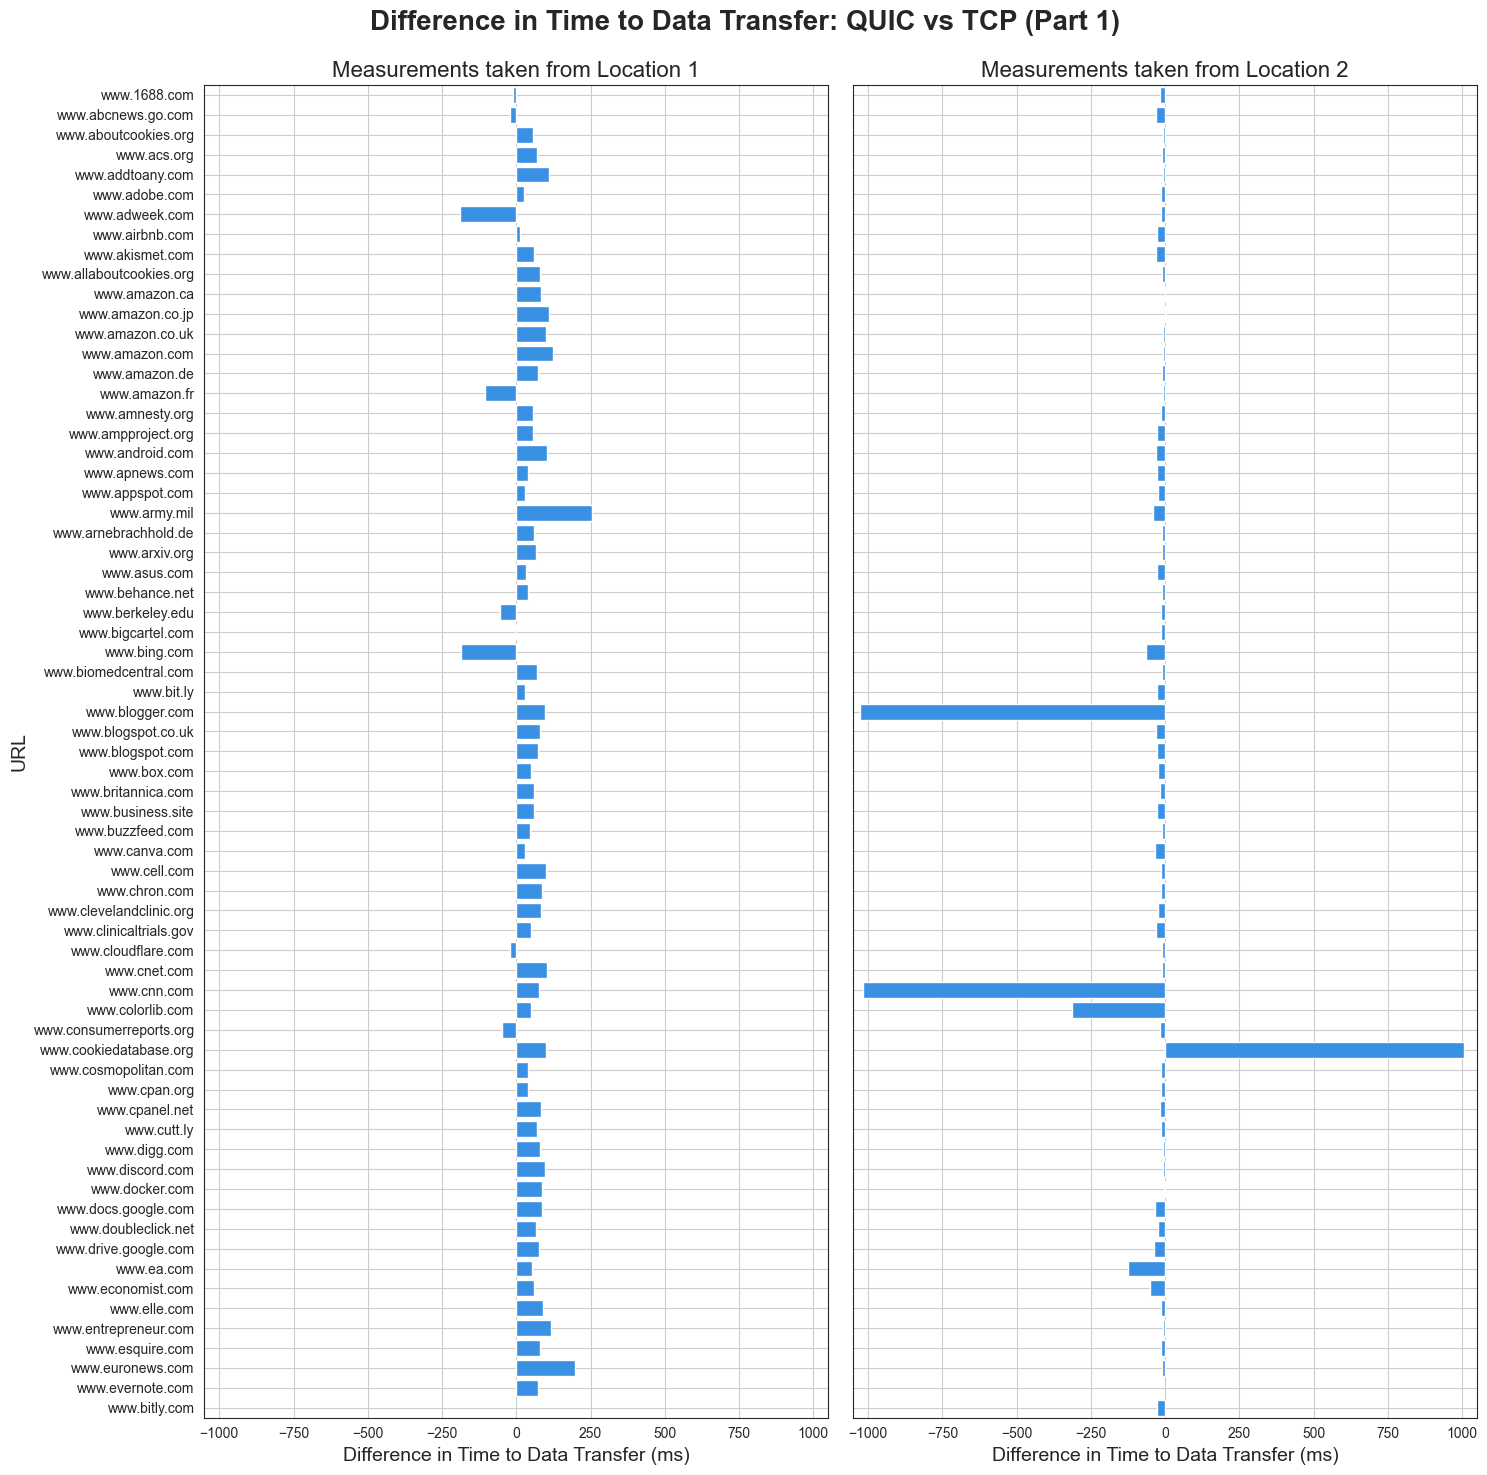
\includegraphics[width=1\linewidth]{images/urlDifference_QUICvsTCP_part1.png}
    \caption{A bar graph depicting difference in time taken before being able to transfer data using both QUIC and TCP. A positive value indicates that QUIC was faster than TCP, while a negative value indicates the opposite. The graph on the left shows data collected at Location 1, while the one on the right shows data collected at Location 2. This figure contains the first 1/4 of the total data collected.}
    \label{fig:urlDifference_p1}
\end{figure}

\begin{figure}
    \centering
    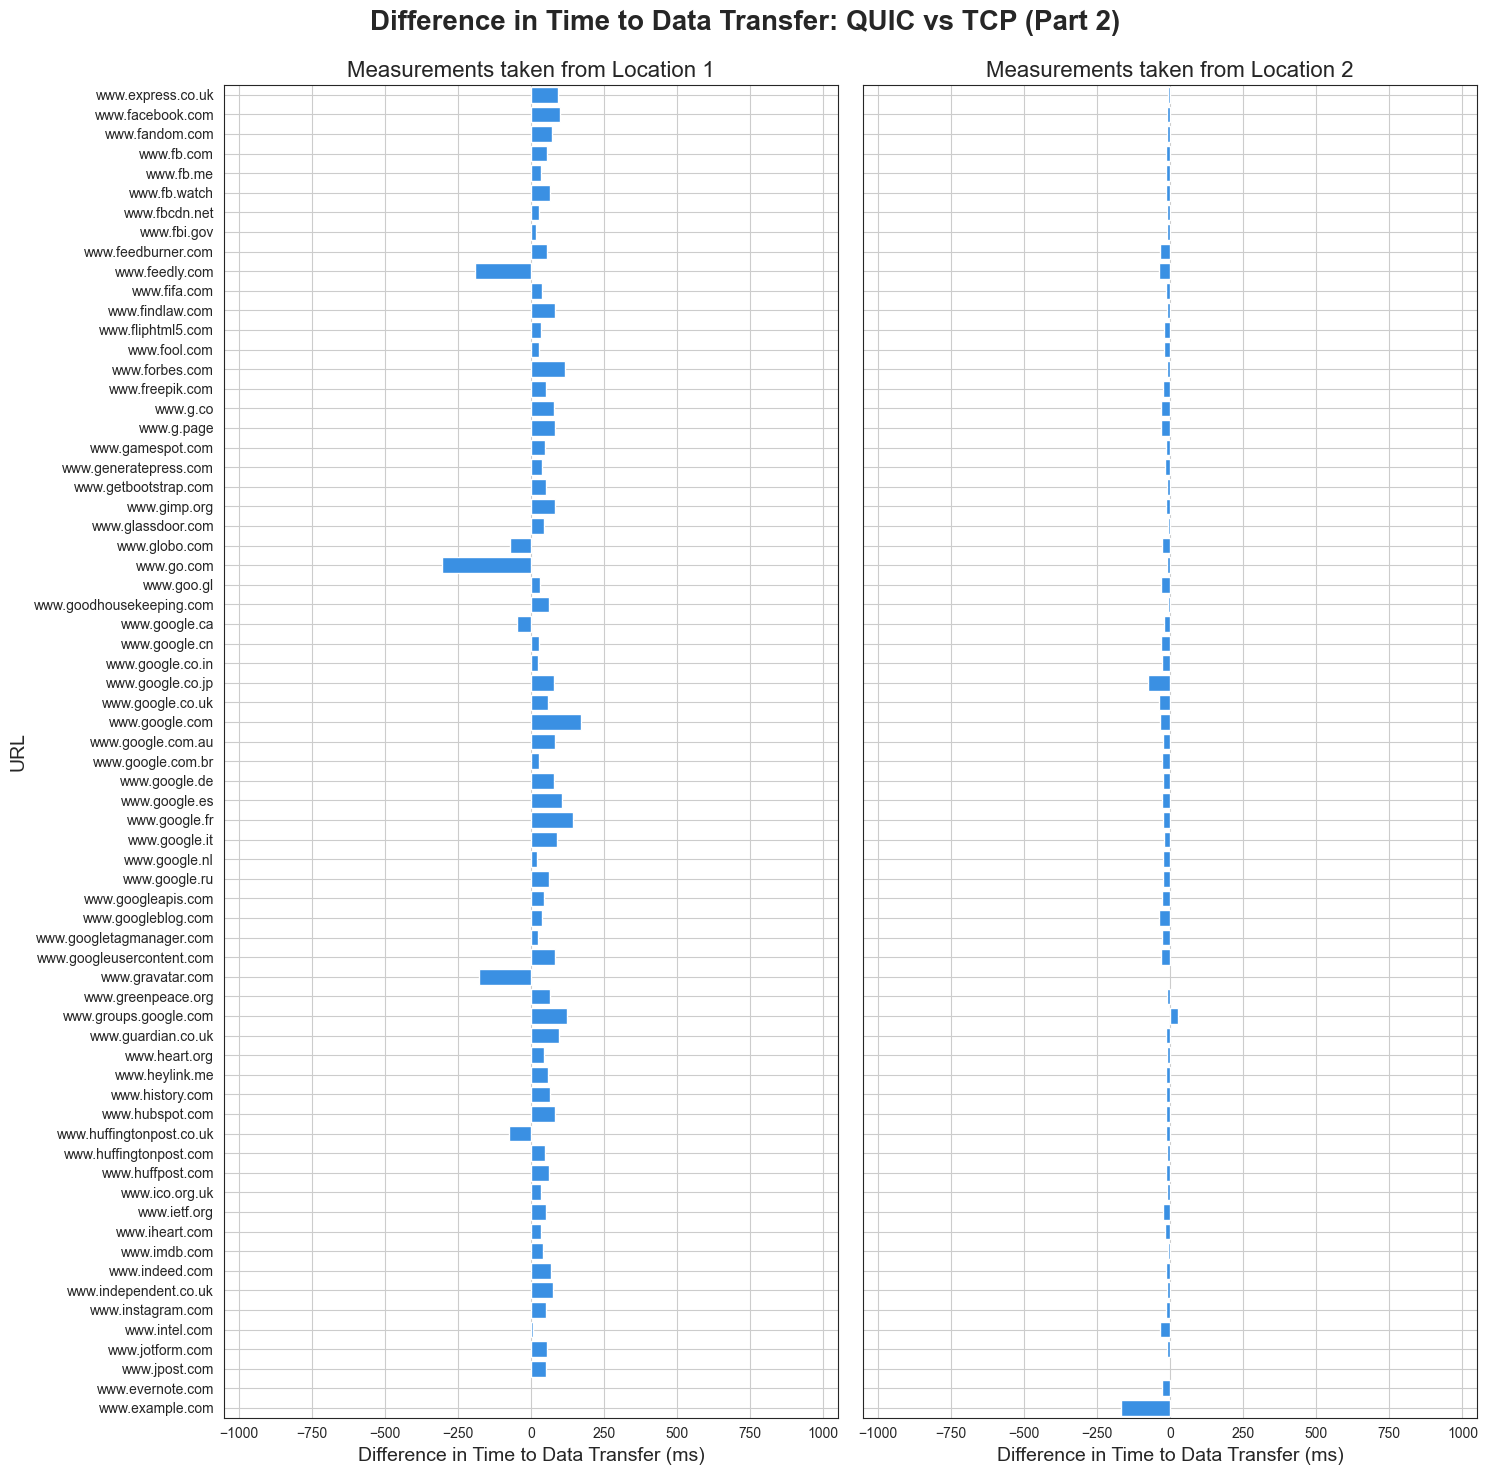
\includegraphics[width=1\linewidth]{images/urlDifference_QUICvsTCP_part2.png}
    \caption{A bar graph depicting difference in time taken before being able to transfer data using both QUIC and TCP. A positive value indicates that QUIC was faster than TCP, while a negative value indicates the opposite. The graph on the left shows data collected at Location 1, while the one on the right shows data collected at Location 2. This figure represents the second out of four graphs depicting only a quarter of the total data collected.}
    \label{fig:urlDifference_p2}
\end{figure}

\begin{figure}
    \centering
    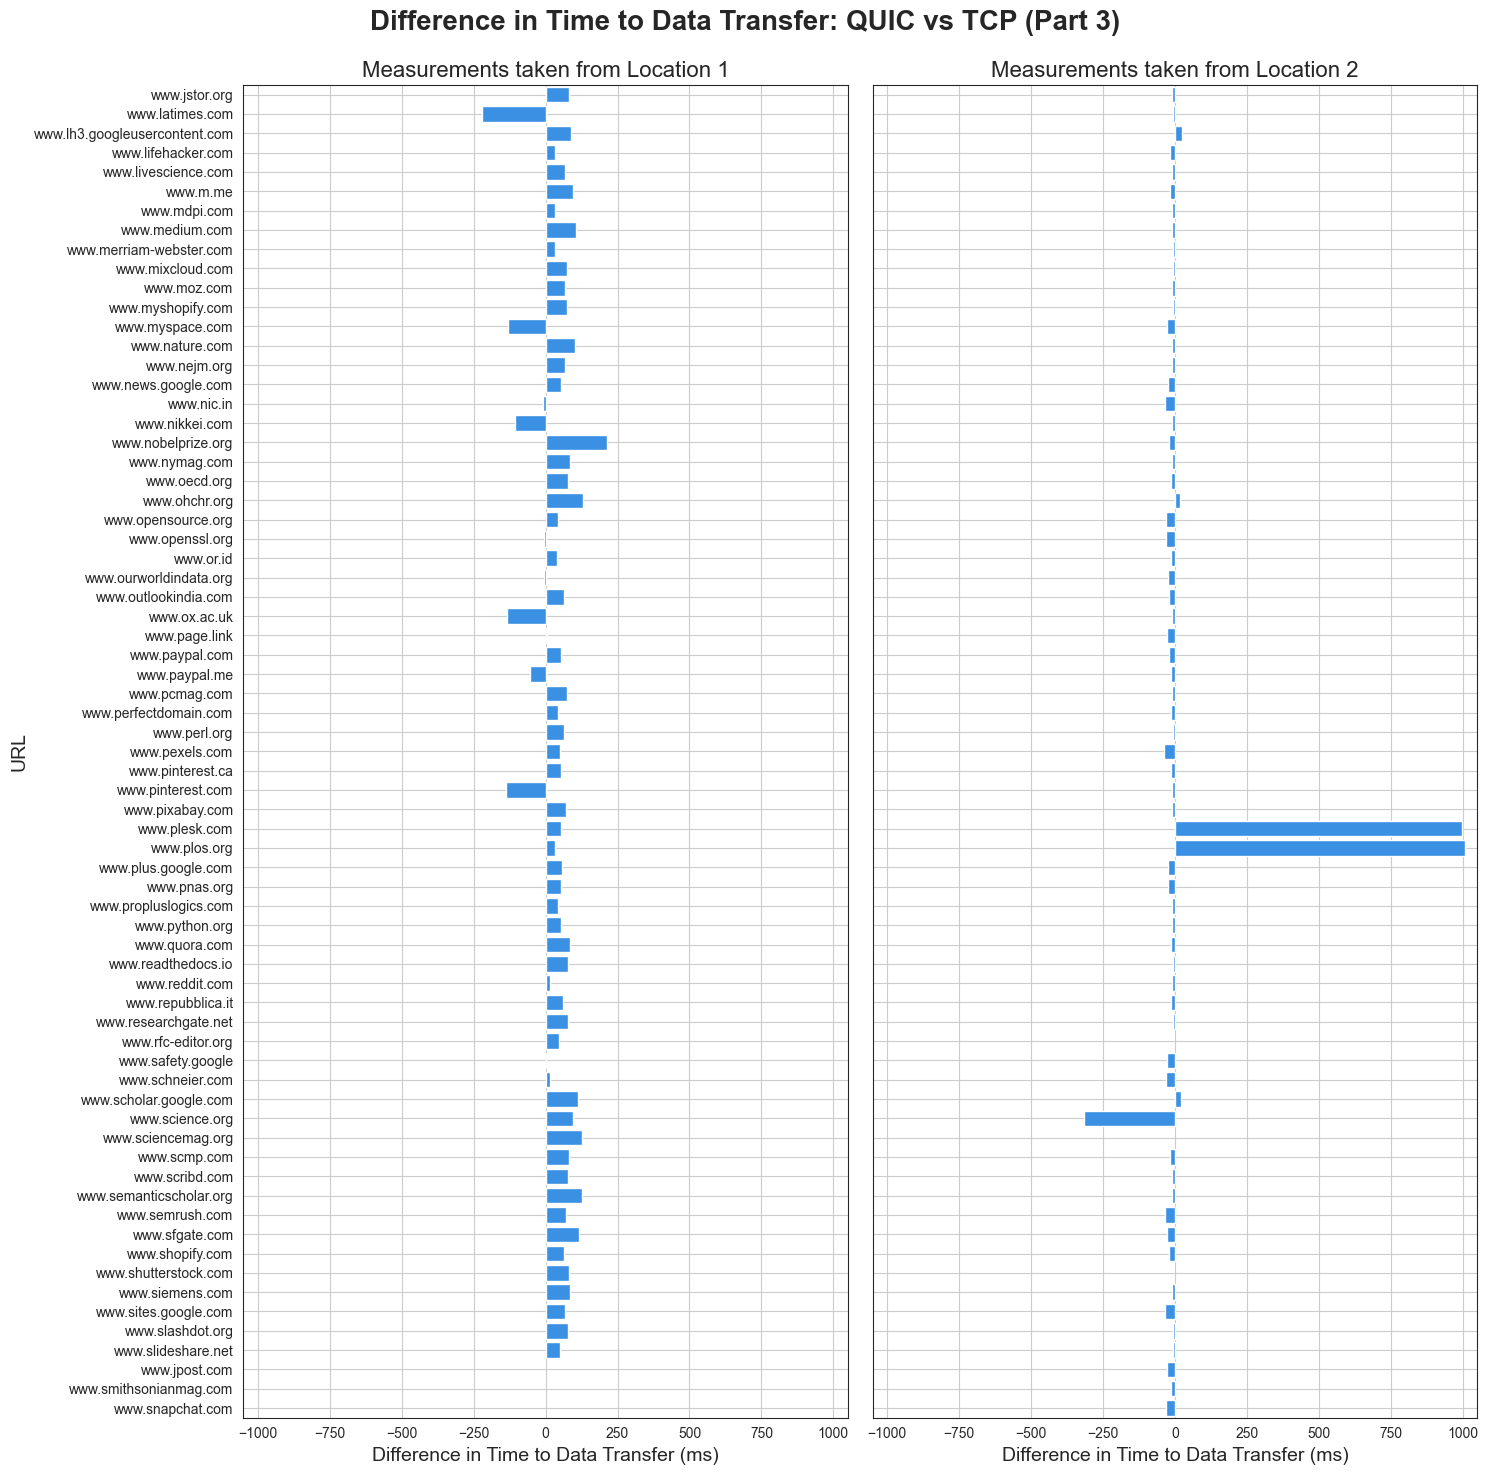
\includegraphics[width=1\linewidth]{images/urlDifference_QUICvsTCP_part3.png}
    \caption{A bar graph depicting difference in time taken before being able to transfer data using both QUIC and TCP. A positive value indicates that QUIC was faster than TCP, while a negative value indicates the opposite. The graph on the left shows data collected at Location 1, while the one on the right shows data collected at Location 2. This figure represents the third out of four graphs depicting only a quarter of the total data collected.}
    \label{fig:urlDifference_p3}
\end{figure}

\begin{figure}
    \centering
    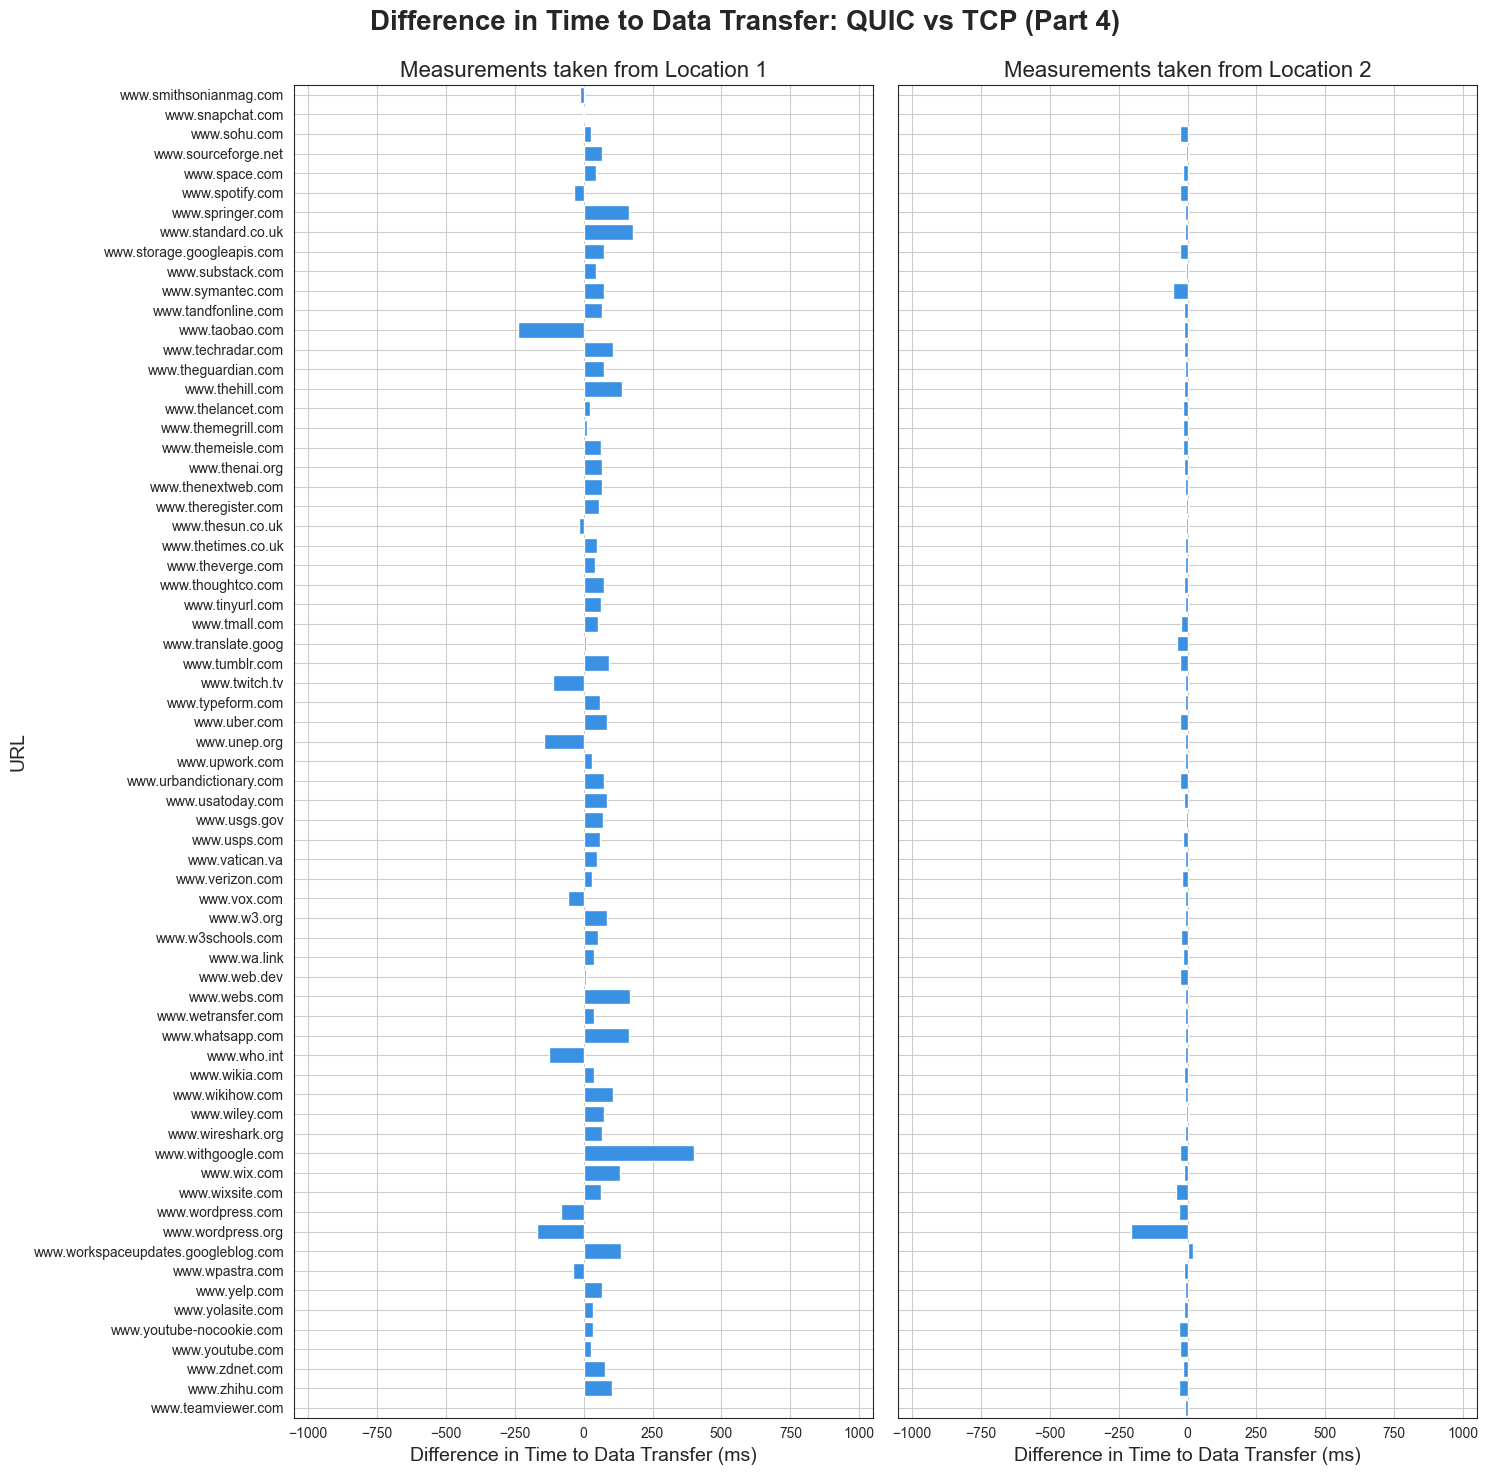
\includegraphics[width=1\linewidth]
    {images/urlDifference_QUICvsTCP_part4.png}
    \caption{A bar graph depicting difference in time taken before being able to transfer data using both QUIC and TCP. A positive value indicates that QUIC was faster than TCP, while a negative value indicates the opposite. The graph on the left shows data collected at Location 1, while the one on the right shows data collected at Location 2. This figure represents the last out of four graphs depicting the final quarter of the total data collected.}
    \label{fig:urlDifference_p4}
\end{figure}


\end{appendices}

%==================================================================================================================================
%   BIBLIOGRAPHY   

\bibliographystyle{agsm}

% Force the bibliography not to be numbered
\renewcommand{\thechapter}{0} 
\bibliography{l4proj}

\end{document}
